\documentclass{homework}

% Palatino for rm and math | Helvetica for ss | Courier for tt
% \usepackage{mathpazo} % math & rm
% \linespread{1.05}        % Palatino needs more leading (space between lines)
\usepackage[scaled]{helvet} % ss
\usepackage{courier} % tt
\normalfont
% \usepackage[T1]{fontenc}
\usepackage{booktabs}
\usepackage{graphicx}
\graphicspath{ {../images/} }
\usepackage{float}
\usepackage{subcaption}

% \usepackage[nottoc]{tocbibind}

\usepackage{biblatex}
\addbibresource{bib.bib}

\usepackage{hyperref}
\usepackage{url}

\Title{Exploration of COVID-19 Data}
\DueDate{April 30, 2020}
\ClassName{Machine Learning Fundamentals and Applications}
\ClassNumber{CS559}
\ClassSection{Spring 2020}
\Instructor{Professor In Suk Jang}
\Author{Daniel Kadyrov}

\begin{document}

\maketitle

\begin{abstract}
  \noindent An analysis on predicting the spread, ending, growth rate and mitigation, weather correlations, of COVID-19 and case study of its effects on New York.
\end{abstract}

\newpage
\thispagestyle{empty}
\tableofcontents

\newpage
\setcounter{page}{1}
\section{Introduction}

Coronavirus disease 2019, COVID-19, is an infectious disease that was first identified in December 2019 at the city of Wuhan, China and has since spread to a worldwide pandemic affecting international politics and economics, changing social interaction as governments mandate stay at home orders, and even becoming the subject of an online machine learning course project.\\

Even though trading restrictions and panic buying have caused a limited amount of medical supplies, like personal protective equipment and respirators, and commodities, such as food staples, cleaning products, and toilet paper, the data on COVID-19 is released and widely available to predict how this virus spreads, when it will end, study the effects of different mitigation types utilized by countries faced with the pandemic, examine if the weather affects the virus spread, and inspect how it behaves in one of the most densely populated and affected cities so far, New York City.

\section{Data}

COVID-19 data was made available by the John Hopkins University Center for Systems Science and Engineering. The dataset is an aggregate of sources that range from the World Health Organization, WHO, COVID Tracking Project, and the health and disease control centers of countries including China, the United States, Italy, Canada, and Taiwan. The dataset was downloaded from Kaggle. \\

New York City, one of the most affected cities in the United States and the world, has made the New York City Department of Health dataset available on Github. Additional data was found on New York City Open Data.\\

All data used for this report was accessed on April 26th 2020.

\subsection{Data Preprocessing}

Data was imported into Python using the \texttt{Pandas} package available through \texttt{Pip}. Column names like \texttt{ObservationDate} and \texttt{Country/Region} were renamed to \texttt{Date} and \texttt{Country}, respectively. Country names listed, such as Mainland China, UK, US, were replaced to reflect their widely used names, China, United States, and United Kingdom, respectively. The serial number column, \texttt{SNo}, was dropped.

\begin{lstlisting}[language=Python, caption={Importing COVID-19 dataset}, firstnumber=12]
import pandas as pd

df = pd.read_csv("../data/novel-corona-virus-2019-dataset/covid_19_data.csv", parse_dates=["Last Update"])
df.rename(columns={ "ObservationDate": "Date",
                    "Country/Region": "Country"}, inplace=True)

df["Country"].replace(["Mainland China"], ["China"], inplace=True)
df["Country"].replace(["US"], ["United States"], inplace=True)
df["Country"].replace(["UK"], ["United Kingdom"], inplace=True)

df = df.drop(columns="SNo")
\end{lstlisting}

\newpage
Continents were added to the data through the package \texttt{Pycountry}.

\begin{lstlisting}[language=Python, caption={Adding continent data}, firstnumber=29]
import pycountry_convert as pc

def get_continent(row):
    continents = {
        'NA': 'North America',
        'SA': 'South America',
        'AS': 'Asia',
        'OC': 'Oceania',
        'AF': 'Africa',
        'EU': 'Europe'
    }

    country = row["Country"]
    try:
        country_code = pc.country_name_to_country_alpha2(
            country, cn_name_format="default")
        return continents[pc.country_alpha2_to_continent_code(country_code)]
    except:
        return None

df["Continent"] = df.apply(lambda row: get_continent(row), axis=1)
\end{lstlisting}

The number of cases of COVID-19 that were eradicated can be found by adding the number of recovered patients with the number of deaths.

\begin{equation}
  N_{\text{eradicated}} = N_{\text{deaths}} + N_{\text{recovered}}
\end{equation}

The number of active cases of COVID-19 can be found by subtracting the number of eradicated cases from the number of confirmed cases.

\begin{equation}
  N_{\text{active}} = N_{\text{confirmed}} - N_{\text{eradicated}}
\end{equation}

\begin{lstlisting}[language=Python, caption={Computed eradicated and active cases}, firstnumber=25]
df["Eradicated"] = df["Deaths"] + df["Recovered"]
df["Active"] = df["Confirmed"] - df["Eradicated"]
\end{lstlisting}

\newpage
\subsection{Exploration of Data}

Table \ref{Continent Spread} shows the prolific spread of the virus throughout the inhabitant continents of the world.

\begin{table}[h]
  \caption{Spread of COVID-19 by Continent}
  \label{Continent Spread}
  \centering
  \begin{tabular}{lrrrrrr}
    \toprule
    Continent     & Confirmed & Deaths & Recovered & Eradicated & Active \\
    \midrule
    Europe        & 1,251,929   & 120,150 & 407,130    & 527,280     & 724,649 \\
    North America & 1,013,138   & 58,224  & 125,756    & 183,980     & 829,158 \\
    Asia          & 460,182    & 16,946  & 220,668    & 237,614     & 222,568 \\
    South America & 131,250    & 47,826  & 6,019      & 53,845      & 77,405  \\
    Africa        & 29,683     & 9,013   & 1,341      & 10,354      & 19,329  \\
    Oceania       & 8,190      & 98     & 5,375      & 5,473       & 2,717   \\
    \bottomrule
  \end{tabular}
\end{table}

Visualizing the confirmed cases over time shows how fast this virus grew in a months time.

\begin{figure}[h]
  \centering
  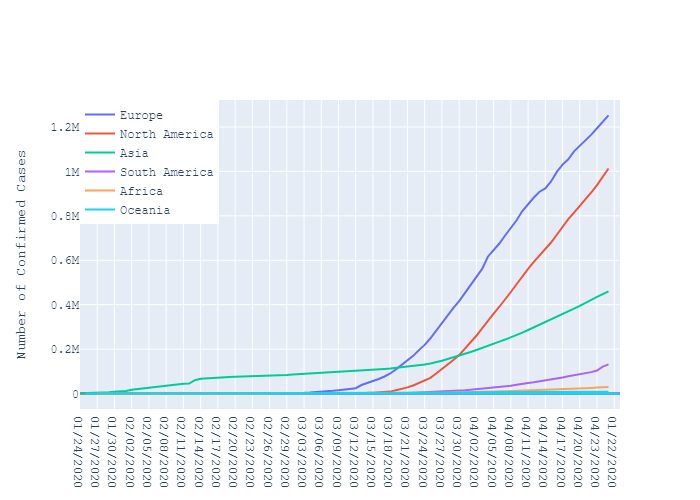
\includegraphics[scale=0.6]{continent}
  \caption{Spread of COVID 19 by Continent}
\end{figure}

\newpage

Analyzing the top countries with confirmed cases by continent:

\begin{table}[H]
  \caption{Spread of COVID-19 in Europe}
  \label{Europe Spread}
  \centering
  \begin{tabular}{lrrrrr}
    \toprule
    Country & Confirmed & Deaths & Recovered & Eradicated & Active \\
    \midrule
    Italy   & 195,351    & 26,384  & 63,120     & 89,504      & 105,847 \\
    Spain   & 223,759    & 22,902  & 95,708     & 118,610     & 105,149 \\
    Germany & 156,513    & 5,877   & 109,800    & 115,677     & 40,836  \\
    \bottomrule
  \end{tabular}
\end{table}

\vspace{-1.5em}

\begin{table}[H]
  \caption{Spread of COVID-19 in North America}
  \label{North America Spread}
  \centering
  \begin{tabular}{lrrrrr}
    \toprule
    Country       & Confirmed & Deaths & Recovered & Eradicated & Active \\
    \midrule
    United States & 938,154    & 53,755  & 100,372    & 154,127     & 784,027 \\
    Canada        & 45,493     & 2,549   & 16,013     & 18,562      & 26,931  \\
    Mexico        & 13,842     & 1,305   & 7,149      & 8,454       & 5,388   \\
    \bottomrule
  \end{tabular}
\end{table}

\vspace{-1.5em}

\begin{table}[H]
  \caption{Spread of COVID-19 in Asia}
  \label{Asia Spread}
  \centering
  \begin{tabular}{lrrrrr}
    \toprule
    Country & Confirmed & Deaths & Recovered & Eradicated & Active \\
    \midrule
    China   & 82,827     & 4,632   & 77,394     & 82,026      & 801    \\
    Iran    & 89,328     & 5,650   & 68,193     & 73,843      & 15,485  \\
    Turkey  & 107,773    & 2,706   & 25,582     & 28,288      & 79,485  \\
    \bottomrule
  \end{tabular}
\end{table}

\vspace{-1.5em}

\begin{table}[H]
  \caption{Spread of COVID-19 in Africa}
  \label{Africa Spread}
  \centering
  \begin{tabular}{lrrrrr}
    \toprule
    Country      & Confirmed & Deaths & Recovered & Eradicated & Active \\
    \midrule
    South Africa & 4,361      & 86     & 1,473      & 1,559       & 2,802   \\
    Egypt        & 4,319      & 307    & 1,114      & 1,421       & 2,898   \\
    Algeria      & 3,256      & 419    & 1,479      & 1,898       & 1,358   \\
    \bottomrule
  \end{tabular}
\end{table}

\vspace{-1em}

\begin{table}[H]
  \caption{Spread of COVID-19 in Oceania}
  \label{Oceania Spread}
  \centering
  \begin{tabular}{lrrrrr}
    \toprule
    Country     & Confirmed & Deaths & Recovered & Eradicated & Active \\
    \midrule
    Australia   & 6,694      & 80     & 4,223      & 4,303       & 2,391   \\
    New Zealand & 1,470      & 18     & 1,142      & 1,160       & 310    \\
    Fiji        & 18        & 0      & 10        & 10         & 8      \\
    \bottomrule
  \end{tabular}
\end{table}


\newpage
\section{Predicting COVID-19 Spread through Interpolation}

\subsection{Methodology}

\subsubsection{Training and Test Data}

Since the data provided is time dependant and the task is to build models to predict the spread of the virus, the training data was set to be all data available until March 31st, 2020 and everything after was used as test data to score the model. This split was created in Python through the following \texttt{Dataframe} manipulation:

\begin{lstlisting}[language=Python, caption={Training and Test Data Split}, firstnumber=153]
x = data.loc[(data['Date'] < "04/01/2020")]["Days"]
y = data.loc[(data['Date'] < "04/01/2020")]["Confirmed"]

x2 = data.loc[(data['Date'] >= "04/01/2020")]["Days"]
y2 = data.loc[(data['Date'] >= "04/01/2020")]["Confirmed"]
\end{lstlisting}

\subsubsection{Exponential Regression}

An exponential model describes the growth of the virus as ever growing and unstoppable. The generic model of the exponential function is:

\begin{equation}
  f(x, a, b, c) = a e^{b(x-c)}
\end{equation}

This was achieved in Python using the curve fit function of the Sklearn library.

\begin{lstlisting}[language=Python, caption={Exponential Model}, firstnumber=149]
from scipy.optimize import curve_fit

def exponential(x, a, b, c):
  return a*np.exp(b*(x-c))

params, corr = curve_fit(exponential, x, y, p0=[0, 0, 0])
y_pred = exponential(x2, *param)
\end{lstlisting}

\subsubsection{Quadratic Regression}

The quadratic model describes the growth of the virus as parabolic. The growth hits an extreme point at the vertex and symmetrically decays at the same rate. The model of the quadratic function is:

\begin{equation}
  f(x, a, b, c) = ax^2 + bx + c
\end{equation}

Within Python:

\begin{lstlisting}[language=Python, caption={Quadratic Model}, firstnumber=168]
from scipy.optimize import curve_fit
  
def quadratic(x, a, b, c):
  return a*(x**2.0) + b*x + c
  
params, corr = curve_fit(quadratic, x, y, p0=[1, 1, 1])

y_pred = quadratic(x2, *param)
\end{lstlisting}

\subsubsection{Logistic Regression}

The logistic function can be appropriately used in modeling the spread of the virus because it captures the growth rate of the exponential function with the assumption that at some point, the inflection point, the rate will decrease until it reaches 1. \\

The logistic function formula is provided as:

\begin{equation}
  f(x, L, k, x_0) = \frac{L}{1+e^{-k(x-x_0)}}
\end{equation}

where $L$ is the curve's maximum value, or scale, $k$ is the logistic growth rate, and $x_0$ is the value of the sigmoid's midpoint \cite{albon_2018}.\\

The logistic function requires for the data to be normalized. A scalar value is generated by assuming the last available y-value, or confirmed case number, is the highest point.

\begin{lstlisting}[language=Python, caption={Logistic Model}, firstnumber=187]
from scipy.optimize import curve_fit
    
def logistic(x, L, k, x0):
  return L/(1+np.exp(-k*(x-x0)))
    
scale = y[-1]
params, corr = curve_fit(logistic, x, y/scale, p0=[1, 1, 1])
  
y_pred = quadratic(x2, *params) * scale
\end{lstlisting}

\subsubsection{Accuracy}

The accuracy of the models was determined through the coefficient of determination, usually denoted as $R^2$. The regression score function was provided by the \texttt{Sklearn} metrics package. A score of 1 denotes the best possible score.

\begin{equation}
  R^2(y, \hat{y}) = 1-\frac{\sum_{i=1}^n(y_i - \hat{y_i})^2}{\sum_{i=1}^{n}(y_i - \bar{y})^2}
\end{equation}

where

\begin{equation*}
  \bar{y} = \frac{1}{n}\sum_{i=1}^{n} y_i
\end{equation*}

\begin{equation*}
  \sum_{i=1}^n(y_i - \hat{y_i})^2 = \sum_{n=1}^n \epsilon_i^2
\end{equation*}

The accuracy score was calculated for only the predicted April data to analyze how well the models foresaw the growth of the virus in the selected country.

\newpage
\subsection{Results}

Table \ref{Task 1 Results} shows the accuracy results of the different regression models to predict the growth of the virus in the selected country. A score closer to the 1 indicates that the model closer foresees how the virus spread in the month of April using the data provided in earlier months. When the exponential model predicts the growth better than the logistic model, it indicates that the virus is spreading unmitigated. A better score in the logistic model suggests that the virus growth is tapering in the country.

\begin{table}[H]
  \caption{Accuracy of COVID-19 Growth Models}
  \label{Task 1 Results}
  \centering
  \begin{tabular}{lrrr}
    \toprule
    Country       & Exponential   & Quadratic    & Logistic  \\
    \midrule
    Algeria       & -300.685364   & 0.270597     & -0.611431 \\
    Australia     & -22206.120326 & -4.654000    & 0.483841  \\
    Brazil        & -41.483849    & -0.409234    & -1.723298 \\
    Canada        & -623.689052   & -2.110432    & -1.267749 \\
    China         & -11072.352650 & -6109.919897 & -6.996825 \\
    Ecuador       & -45.092106    & 0.474223     & -1.293533 \\
    Egypt         & -5.323196     & -0.203390    & -1.830438 \\
    Fiji          & -25.504067    & -48.947467   & -7.469834 \\
    Germany       & -1429.602431  & -0.291852    & -1.252864 \\
    Iran          & -106.636611   & 0.004569     & 0.856650  \\
    Italy         & -402.243797   & -0.633594    & -1.250733 \\
    Mexico        & -60.177645    & -0.208680    & -0.695200 \\
    New Zealand   & -37083.631615 & -6.055959    & -4.194014 \\
    Peru          & 0.453311      & -0.767787    & -1.306760 \\
    South Africa  & -1247.631391  & -4.674649    & -1.328513 \\
    Spain         & -1560.444295  & 0.184842     & -0.712448 \\
    Turkey        & -9964.226390  & 0.808690     & -1.838440 \\
    United States & -1356.526660  & -2.797616    & -1.677107 \\
    \bottomrule
  \end{tabular}
\end{table}

Even though $R^2$ accuracy is poor for all models, it demonstrates the inability to properly predict how the virus will spread especially when data is limited. It is interesting to note that the logistic model, representing the best case, and the exponential model, representing the worst case, create a boundary region for the growth. Examining the spread and models graphically per country in Figure \ref{fig:task1} clearly shows how some countries, like Australia and Iran, have controlled the virus and reflect a logistic curve while countries like Brazil and Egypt are closer to exponential growth.

\begin{figure}[H]
  \centering
  \begin{subfigure}{0.45\linewidth}
    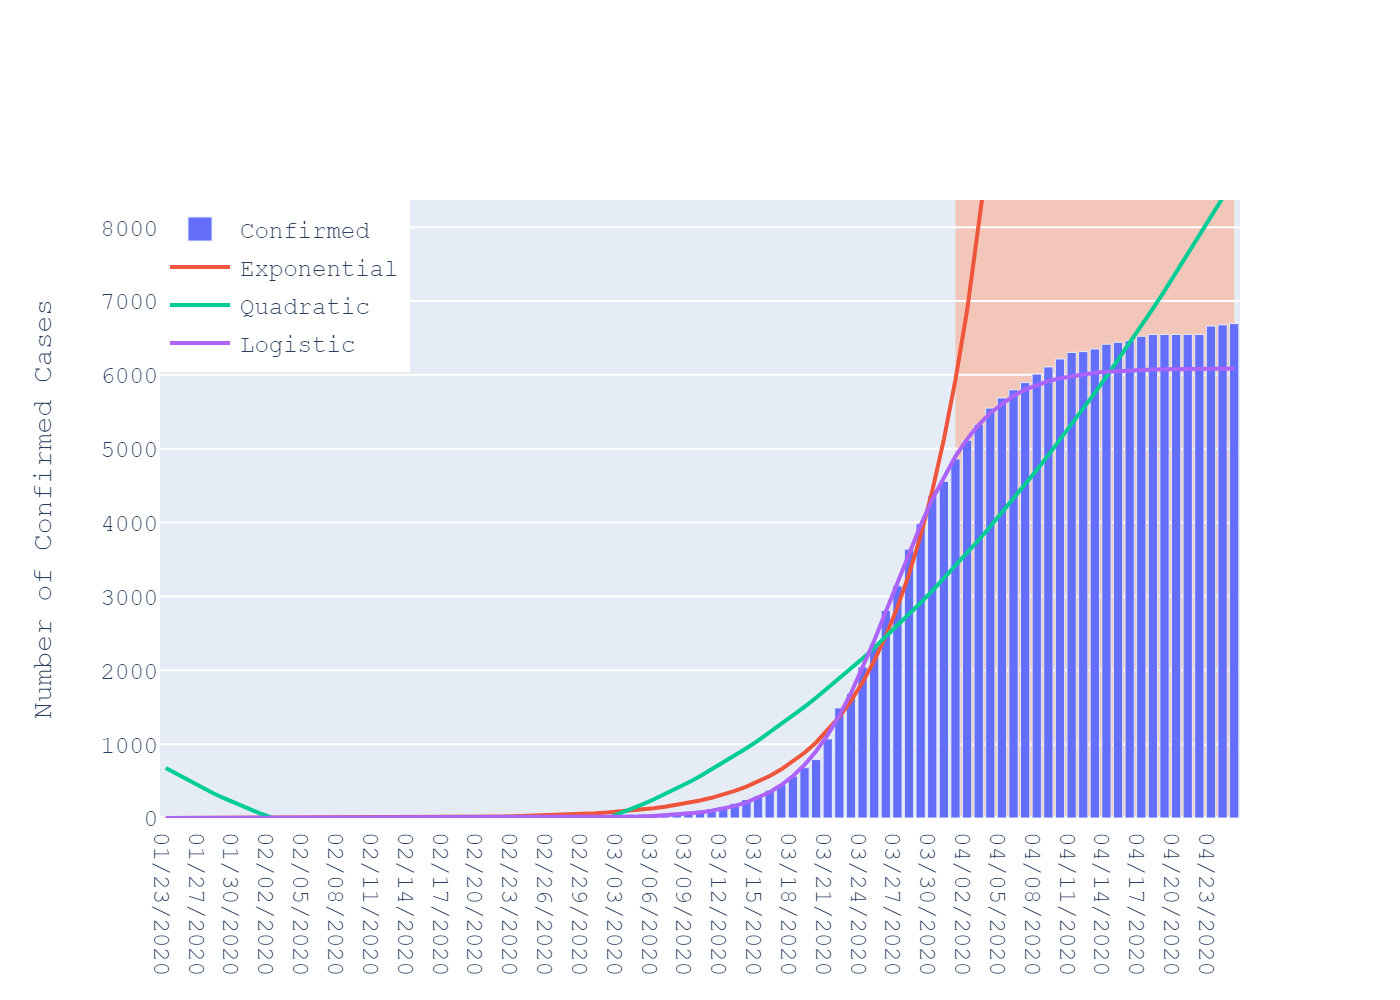
\includegraphics[width=\linewidth]{task1/Australia.png}
    \caption{Australia}
  \end{subfigure}
  \hfil
  \begin{subfigure}{0.45\linewidth}
    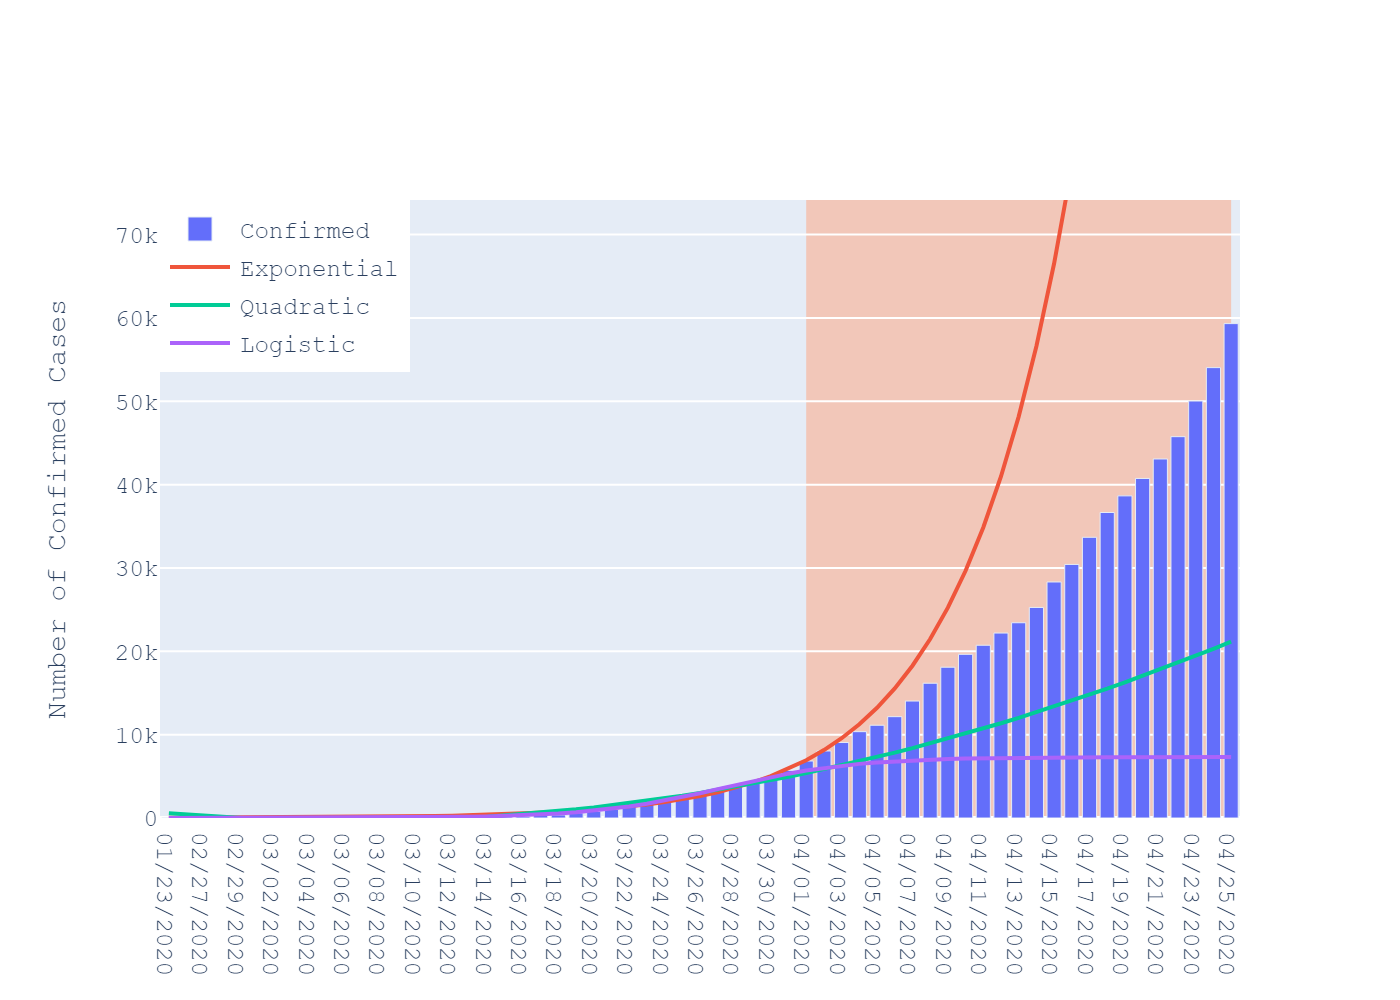
\includegraphics[width=\linewidth]{task1/Brazil.png}
    \caption{Brazil}
  \end{subfigure}

  \begin{subfigure}{0.45\linewidth}
    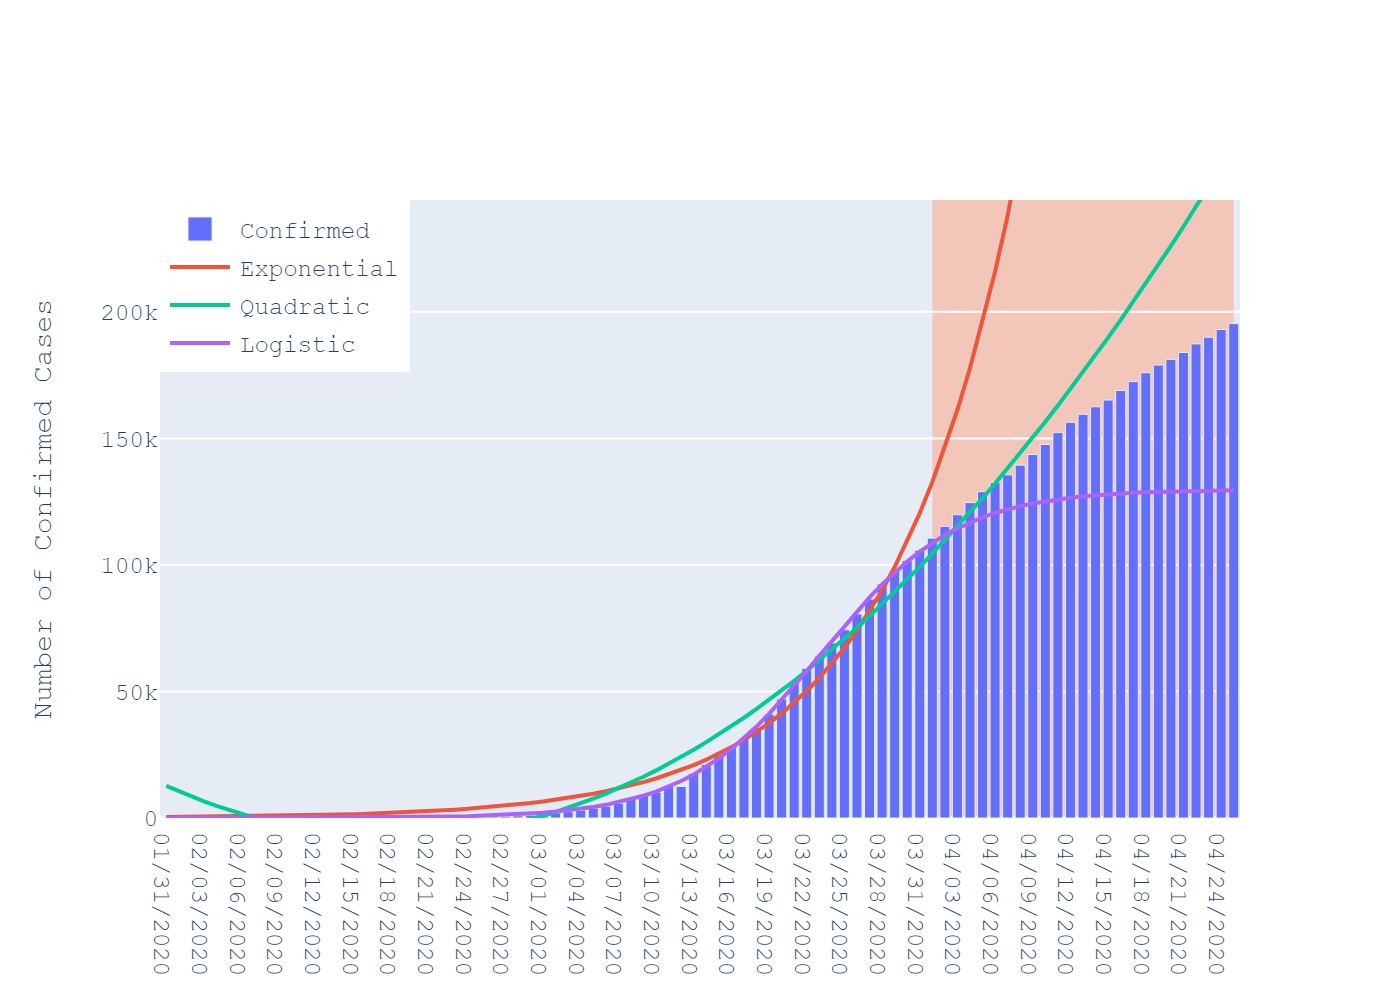
\includegraphics[width=\linewidth]{task1/Italy.png}
    \caption{Italy}
  \end{subfigure}
  \hfil
  \begin{subfigure}{0.45\linewidth}
    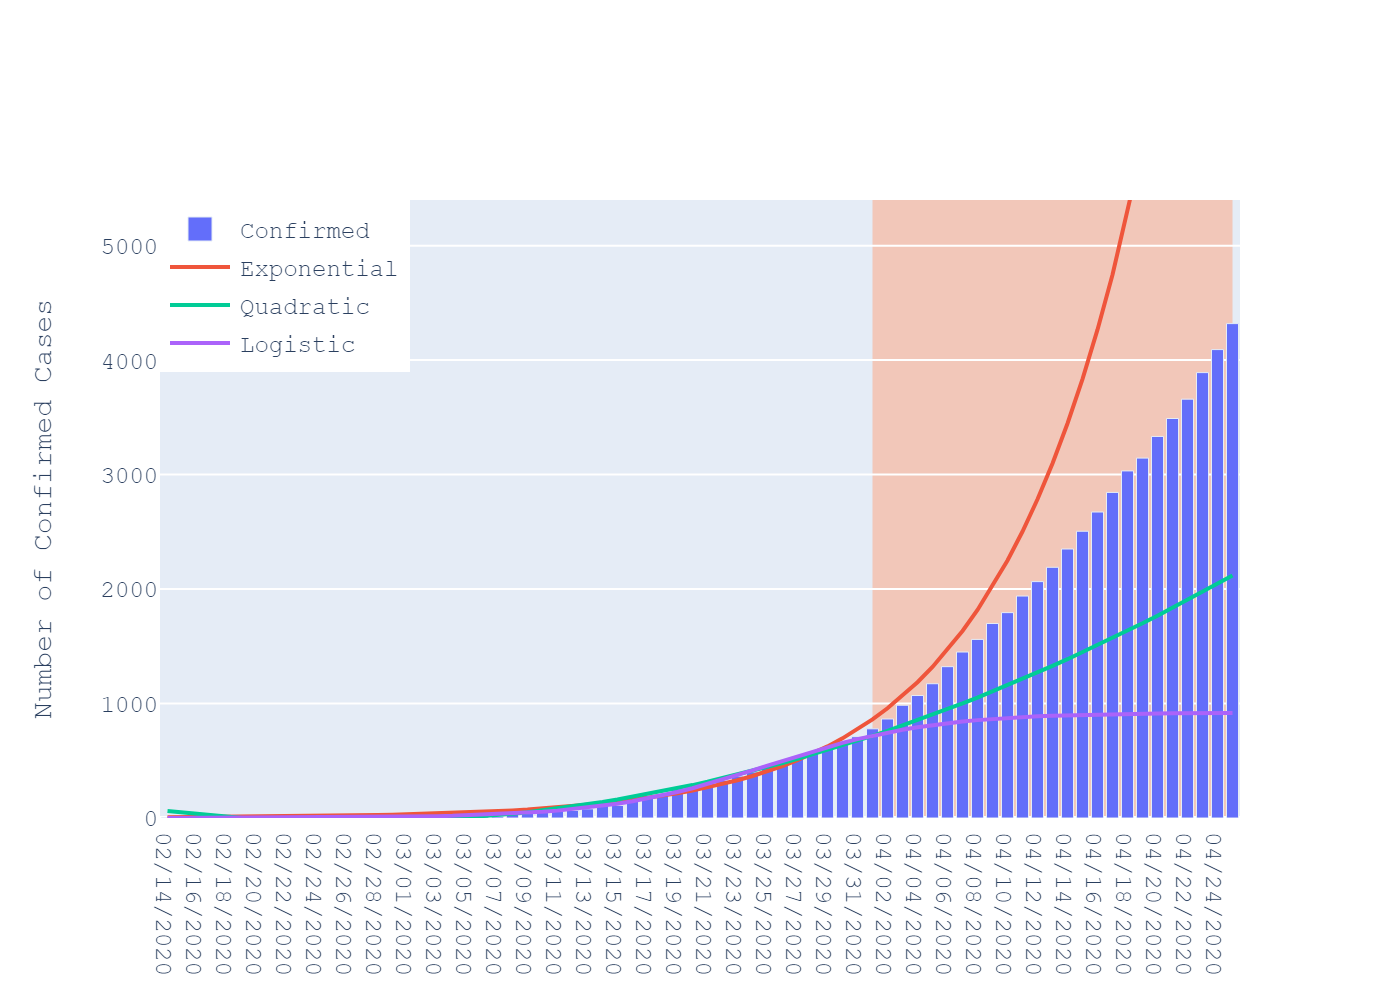
\includegraphics[width=\linewidth]{task1/Egypt.png}
    \caption{Egypt}
  \end{subfigure}

  \begin{subfigure}{0.45\linewidth}
    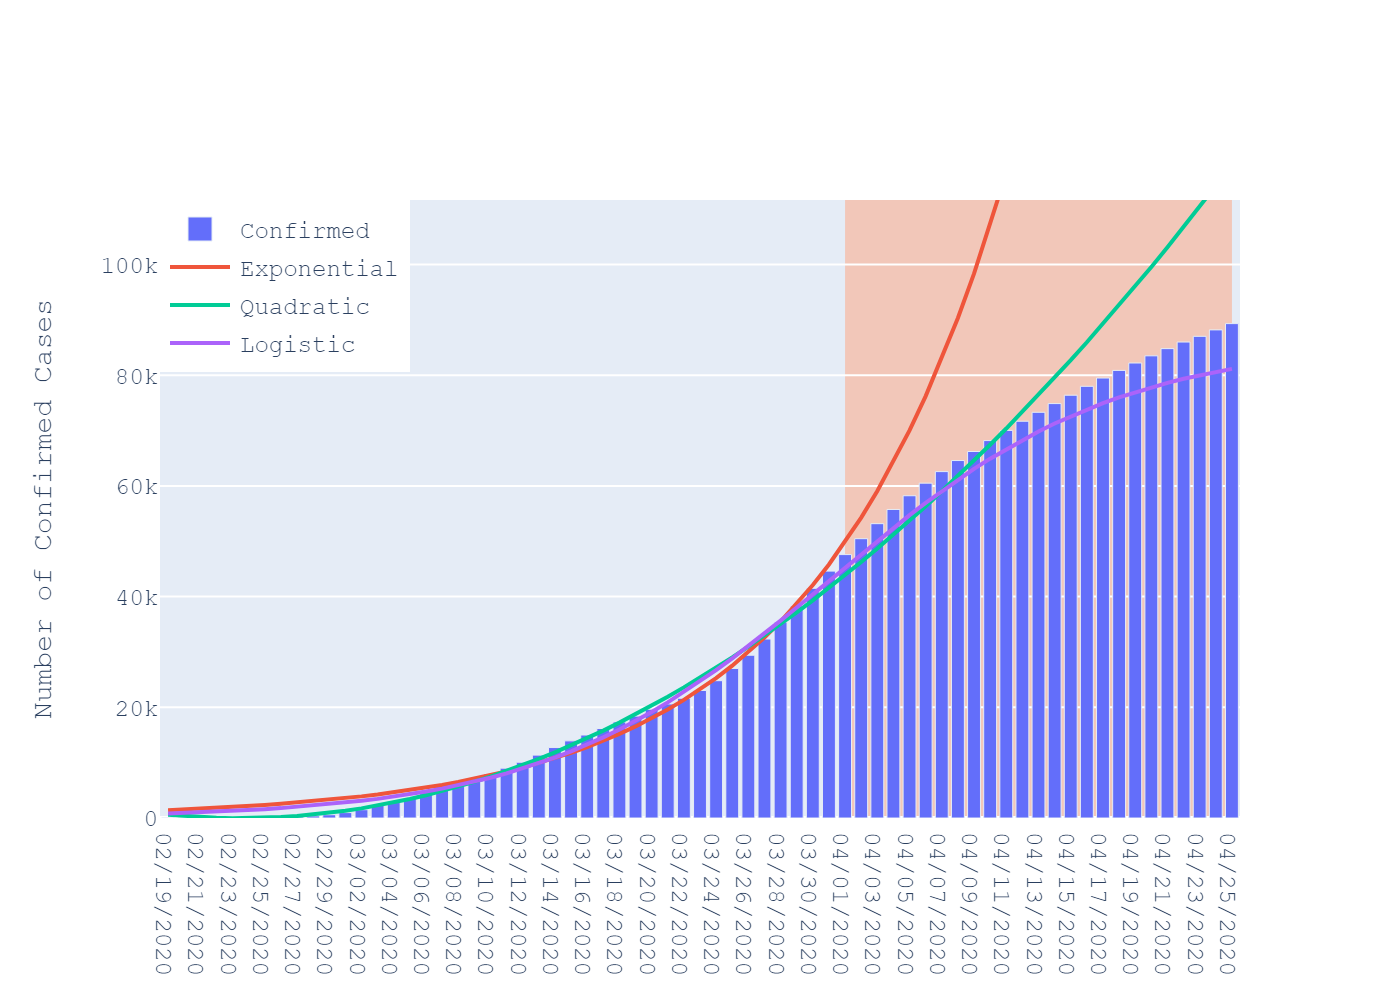
\includegraphics[width=\linewidth]{task1/Iran.png}
    \caption{Iran}
  \end{subfigure}
  \hfil
  \begin{subfigure}{0.45\linewidth}
    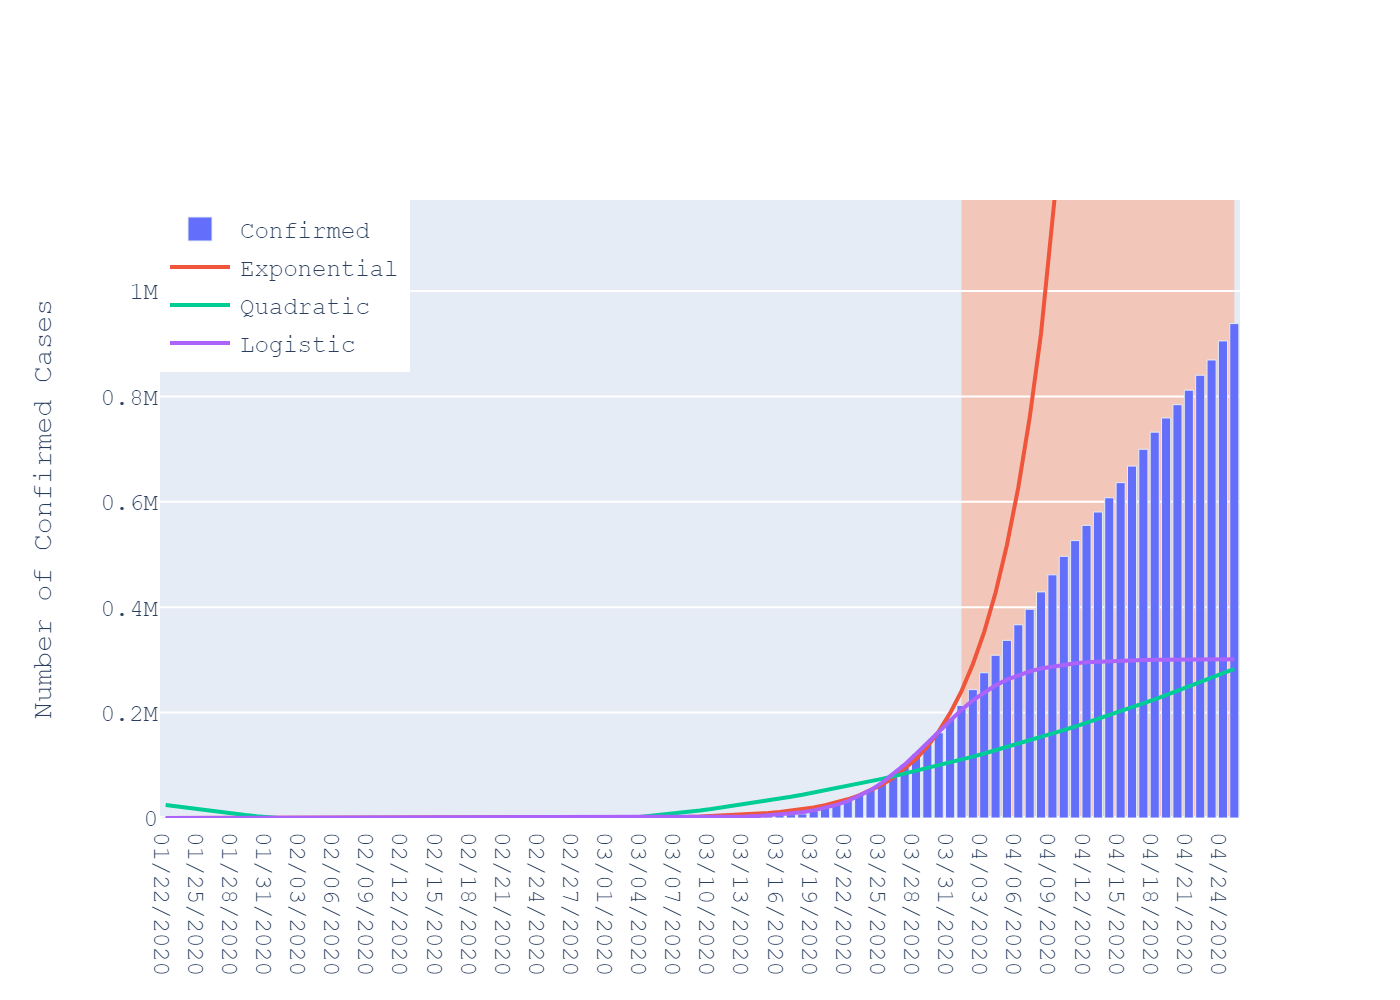
\includegraphics[width=\linewidth]{task1/United States.png}
    \caption{United States}
  \end{subfigure}

  \caption{Modeling COVID-19 Spread}
  \label{fig:task1}
\end{figure}

\newpage
\section{Predicting the End of COVID-19}

\subsection{Methodology}

The logistic model detailed in the previous section captured the growth of the virus until an inflection point during which the growth rate decreases until it gets to 1, a sign that there are no new infections. The pandemic can be determined to be over when the growth rate reaches a certain threshold value which can be found with a ratio between two consecutive logistic functions.

\begin{equation*}
  t = \frac{f(x+1)}{f(x)} = \frac{\frac{L}{1+e^{-k(x+1-x_0)}}}{\frac{L}{1+e^{-k(x-x_0)}}}
\end{equation*}

Rearranging to solve for $x$, when the logistic function reaches the threshold value of $t$.

\begin{equation}
  x = -\frac{1}{k}\log(\frac{1-t}{1e^-k-1}) + x_0
\end{equation}

The threshold value, $t$, was selected to be 1.000001 since using 1 would result in $x$ becoming infinity. The function in Python uses the parameters found in the logistic function.

\begin{lstlisting}[language=Python, caption={Predicting the Last Day}, firstnumber=74]
import numpy as np

def predict_day(params): 
  threshold = 1.000001
  L, k, x0 = params
  last_day = int(round((-1/k)*np.log((1-threshold)/(threshold*np.exp(-k)-1))+x0))

  return last_day
\end{lstlisting}

All available data was used to create the logistic model and was generated for the total confirmed infections and total deaths.

\newpage
\subsection{Results}

Table \ref{Task 2 Results} shows the end date, total confirmed case, and total deaths predicted by the logistic model.

\begin{table}[H]
  \caption{COVID-19 Country End Dates and Total Cases}
  \label{Task 2 Results}
  \centering
  \begin{tabular}{llrr}
    \toprule
    Country       & End Date   & Total Confirmed & Total Deaths \\
    \midrule
    Algeria       & 07/07/2020 & 3,484           & 417          \\
    Australia     & 05/18/2020 & 6,537           & 77           \\
    Brazil        & 06/26/2020 & 98,436          & 6,612        \\
    Canada        & 07/12/2020 & 54,052          & 3,916        \\
    China         & 04/25/2020 & 81,474          & 3,612        \\
    Ecuador       & 01/05/2021 & 1,583,211,969   & 634          \\
    Egypt         & 08/07/2020 & 6,621           & 393          \\
    Germany       & 06/15/2020 & 153,766         & 6,653        \\
    Iran          & 07/13/2020 & 93,834          & 5,714        \\
    Italy         & 07/03/2020 & 193,378         & 26,316       \\
    Mexico        & 07/29/2020 & 115,463         & 7,771        \\
    New Zealand   & 05/23/2020 & 1,446           & 20           \\
    Peru          & 06/29/2020 & 31,963          & 1,771        \\
    South Africa  & 08/26/2020 & 6,468           & 124          \\
    Spain         & 06/21/2020 & 215,326         & 22,369       \\
    Turkey        & 06/24/2020 & 120,058         & 3,258        \\
    United States & 06/30/2020 & 995,581         & 65,028       \\
    \bottomrule
  \end{tabular}
\end{table}

Since the model only uses the data provided up to the date of the simulation, the predictions of some countries, like Ecuador, cannot be completely trusted. As of April 26th, the Institute for Health Metrics and Evaluation projects that the United States will have 67,641 deaths by August 4th \cite{ihme}.\\

Using this model on the total world data generates the following.

\begin{table}[H]
  \caption{COVID-19 World End Date and Total Cases}
  \label{Task 2 Results World}
  \centering
  \begin{tabular}{lrr}
    \toprule
    End Date   & Total Confirmed & Total Deaths \\
    \midrule
    07/29/2020 & 3,440,226       & 250,742      \\
    \bottomrule
  \end{tabular}
\end{table}

\begin{table}[H]
  \caption{COVID-19 Continent End Date and Total Cases}
  \label{Task 2 Results Continent}
  \centering
  \begin{tabular}{llrr}
    \toprule
    Continent     & End Date   & Total Confirmed & Total Deaths \\
    \midrule
    Africa        & 06/02/2020 & 19,432           & 1,103        \\
    Asia          & 02/17/2022 & 31,881,299,685  & 55,866       \\
    Europe        & 06/18/2020 & 106,0795        & 102,298      \\
    North America & 06/08/2020 & 76,6258         & 36,842       \\
    Oceania       & 05/17/2020 & 7,807           & 119          \\
    South America & 05/26/2020 & 98,327          & 3,525        \\
    \bottomrule
  \end{tabular}

\end{table}

\newpage

\begin{figure}[H]
  \centering
  \begin{subfigure}{0.45\linewidth}
    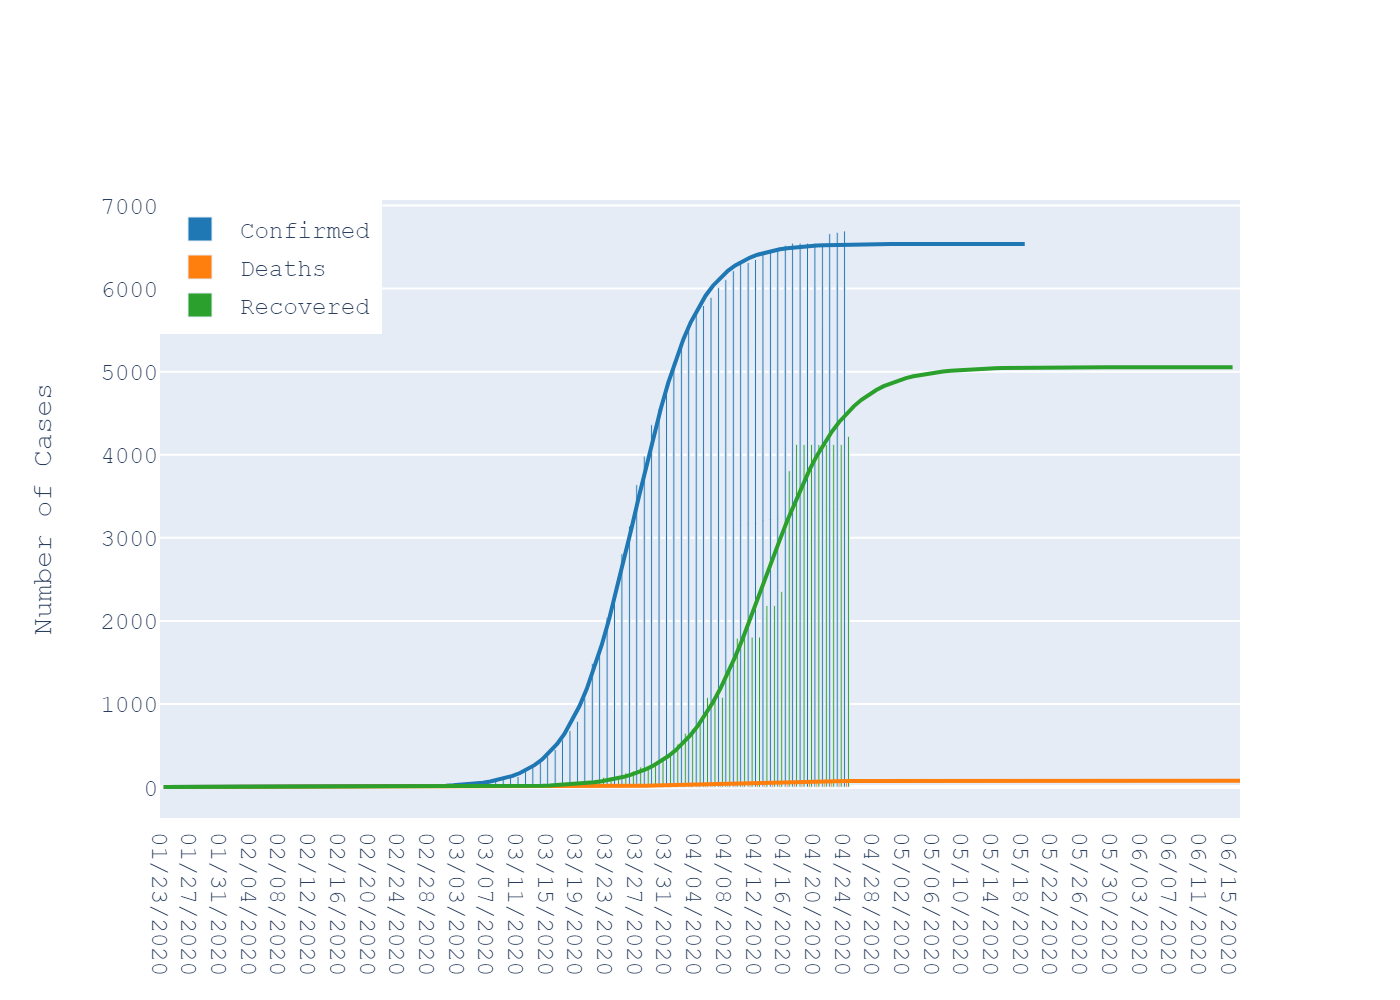
\includegraphics[width=\linewidth]{task2/Australia.png}
    \caption{Australia}
  \end{subfigure}
  \hfil
  \begin{subfigure}{0.45\linewidth}
    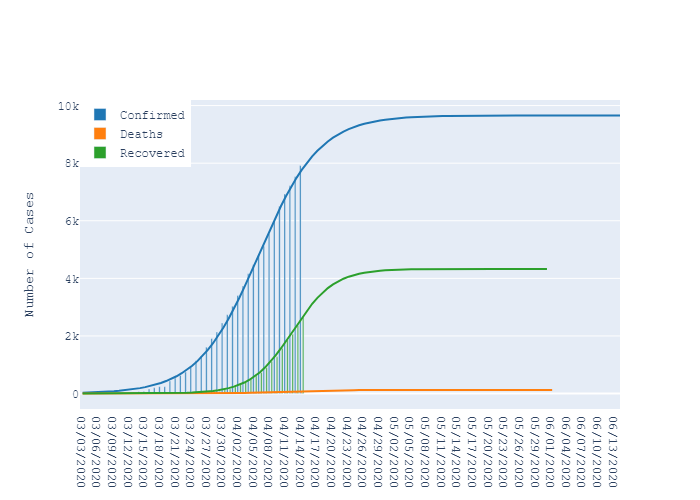
\includegraphics[width=\linewidth]{task2/Chile.png}
    \caption{Ecuador}
  \end{subfigure}

  \begin{subfigure}{0.45\linewidth}
    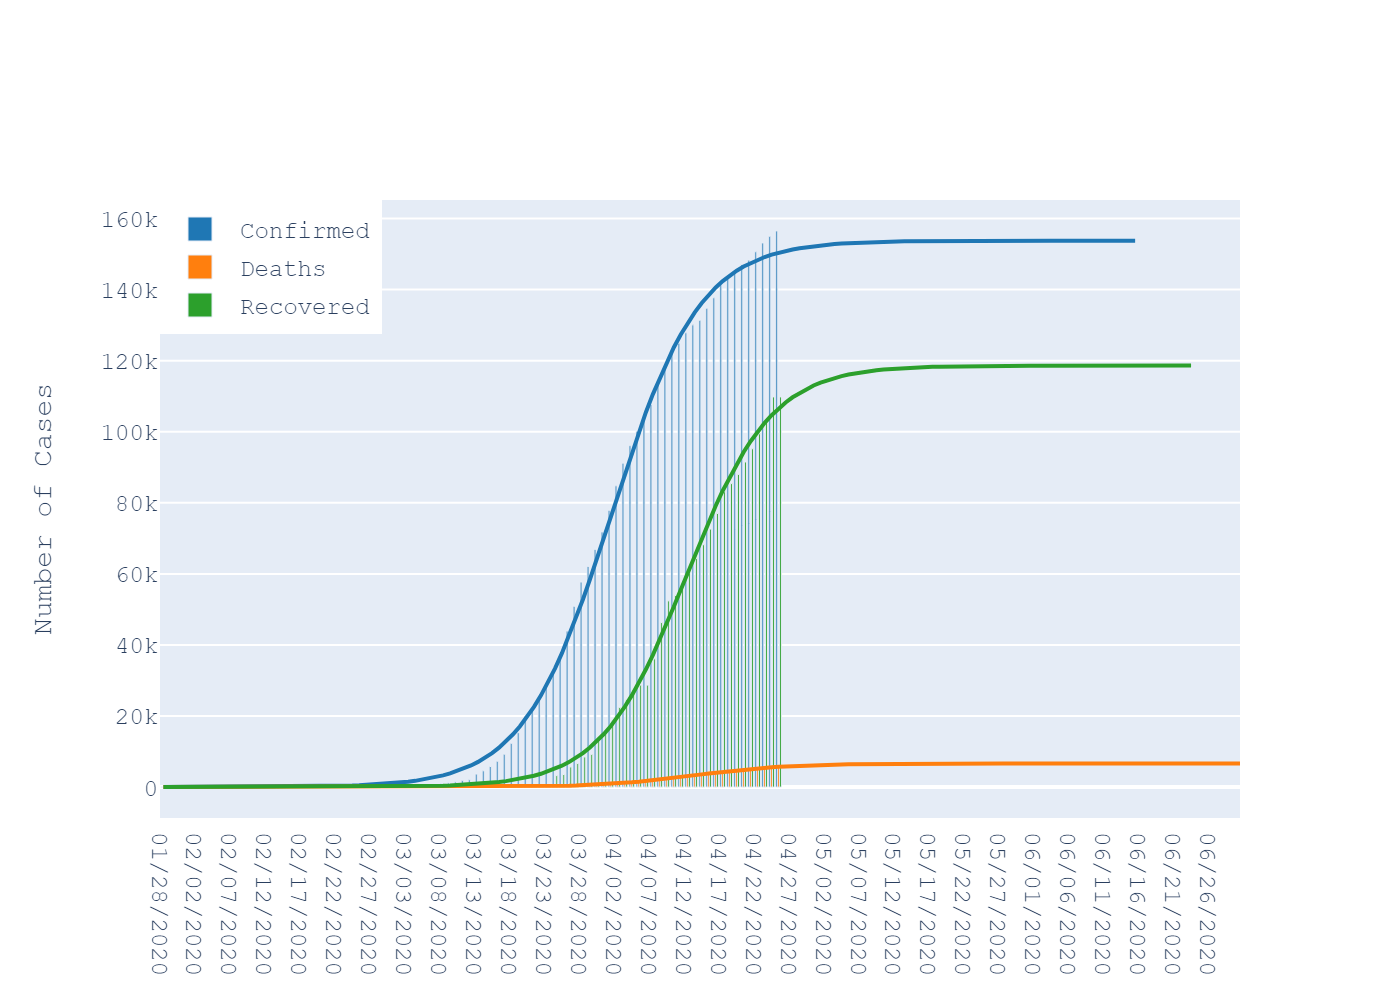
\includegraphics[width=\linewidth]{task2/Germany.png}
    \caption{Germany}
  \end{subfigure}
  \hfil
  \begin{subfigure}{0.45\linewidth}
    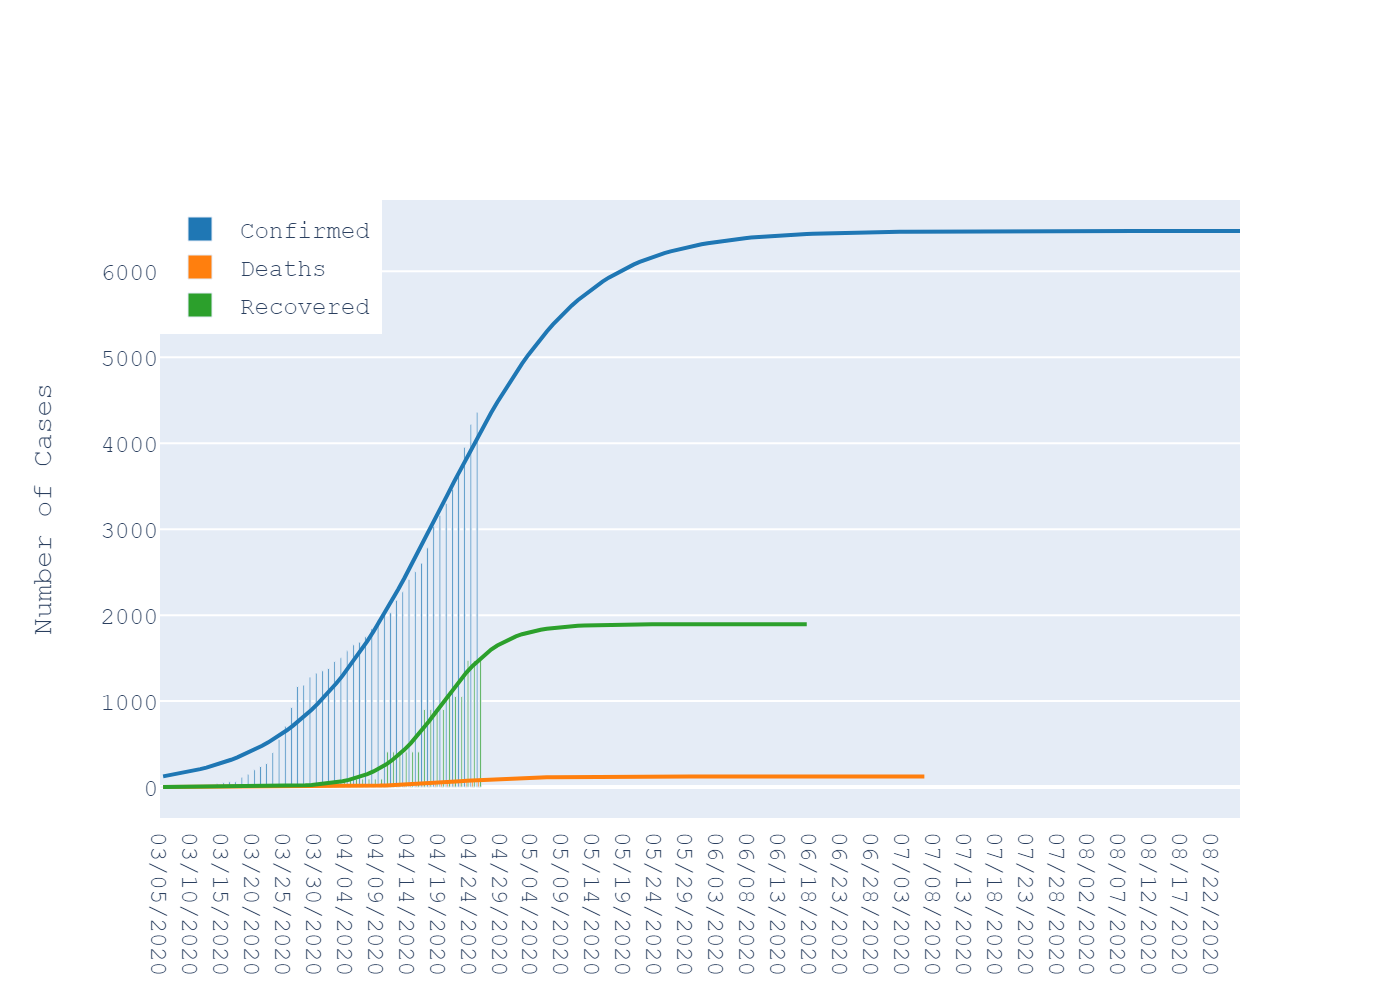
\includegraphics[width=\linewidth]{task2/South Africa.png}
    \caption{South Africa}
  \end{subfigure}

  \begin{subfigure}{0.45\linewidth}
    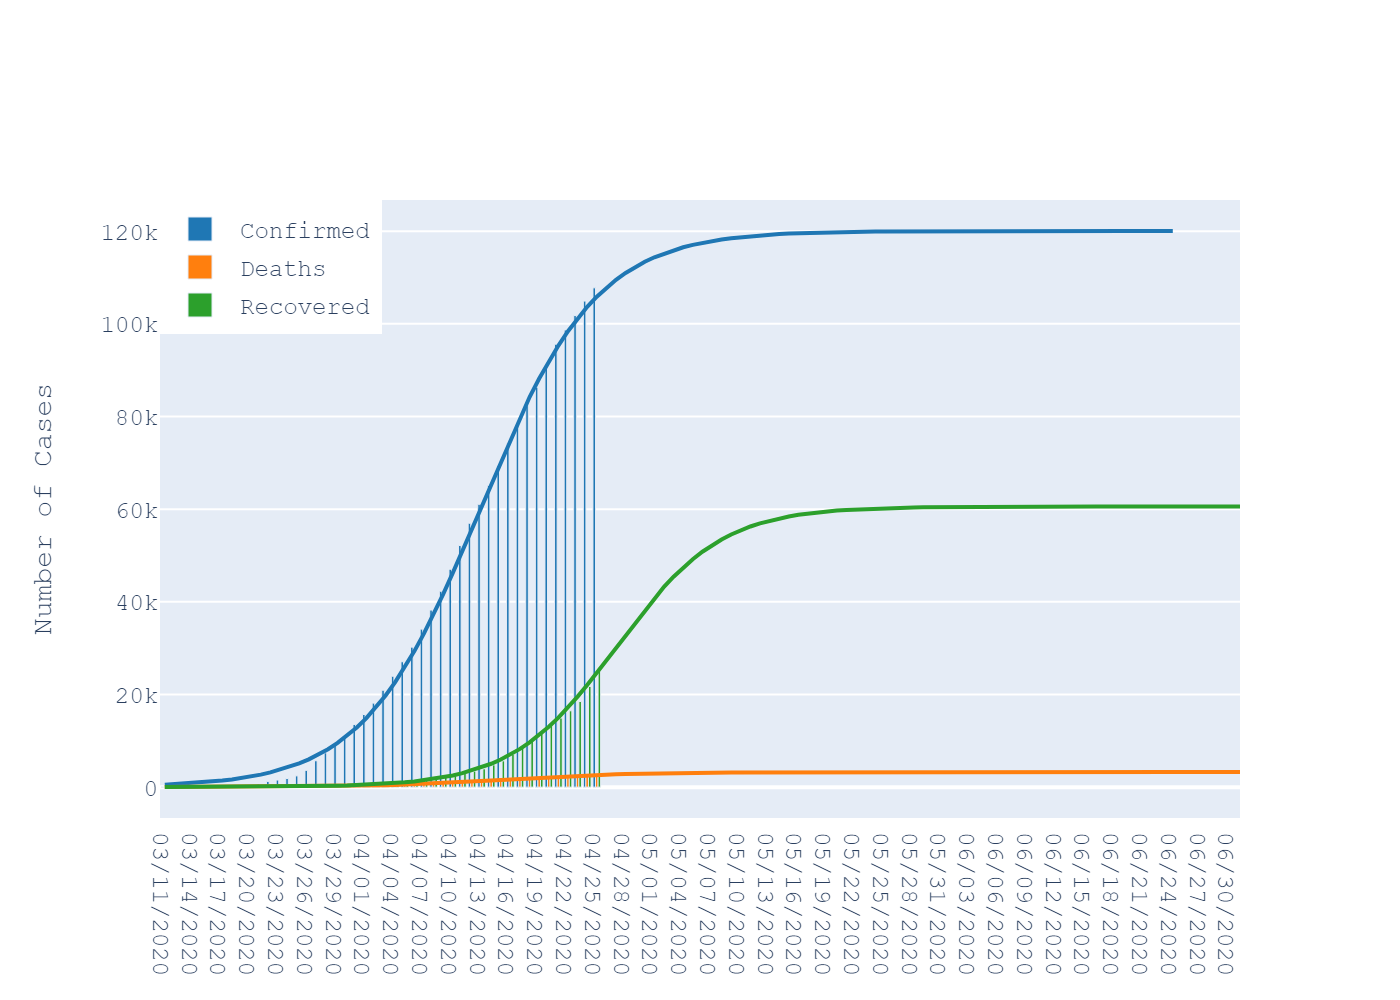
\includegraphics[width=\linewidth]{task2/Turkey.png}
    \caption{Turkey}
  \end{subfigure}
  \hfil
  \begin{subfigure}{0.45\linewidth}
    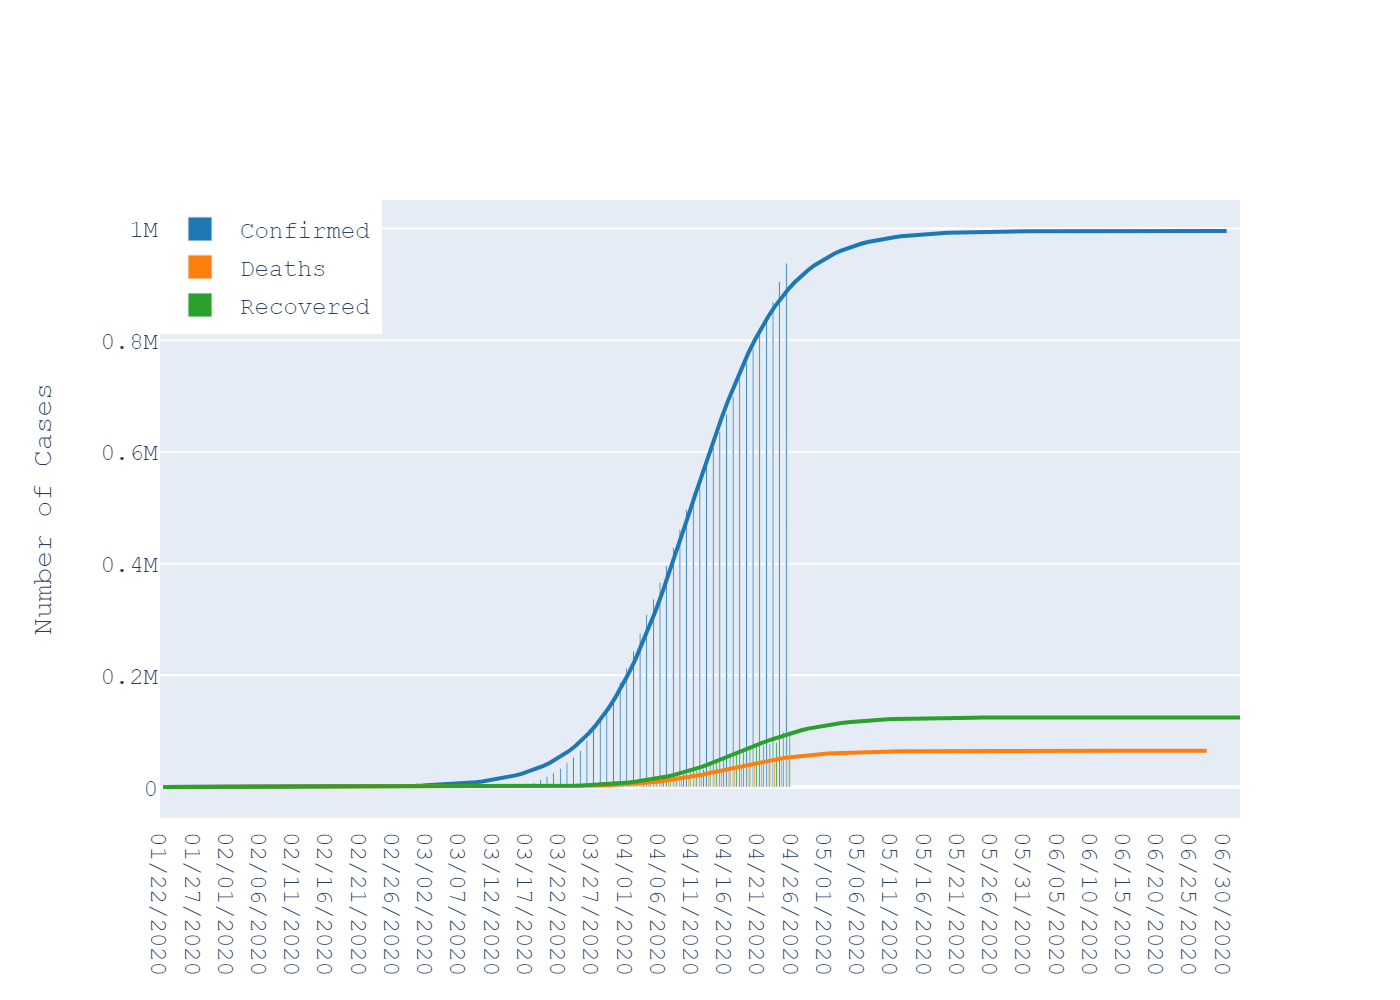
\includegraphics[width=\linewidth]{task2/United States.png}
    \caption{United States}
  \end{subfigure}

  \caption{Predicting the COVID-19 End Date}
  \label{fig:task2}
\end{figure}

\newpage
\section{Types of Mitigation and Growth Rate}
\subsection{Methodology}

The growth rate is a metric of how fast the virus is spreading over a period of time, usually represented as a percentage. The growth rate is defined mathematically as:

\begin{equation}
  \text{GR} = \frac{x_2 - x_1}{\Delta{t}}
\end{equation}

Within Python this was implemented with the following function:

\begin{lstlisting}[language=Python, caption={Growth Rate Function}, firstnumber=56]
def growth_rate(data=None):
  x = []
  x.append(0)
  for i in range(data.shape[0]-1):
      next
      a = abs(data.iloc[i+1]-data.iloc[i])
      if data.iloc[i] == 0:
          v = 0.0
      else:
          v = a/data.iloc[i]
      v=v*100
      x.append(v)
      
  return np.array(x)

df["Growth Rate"] = growth_rate(df["Confirmed"])
\end{lstlisting}

As COVID-19 spread into the confines of various countries, the governments of the respective areas reacted in different ways to mitigate the growth rate of the virus. \\

Using Linear Regression through the Sklearn package, the slope of the growth rate can be found to compare as a metric between different countries. The regression model was created by setting the start point as the date when the growth rate was 1\% of the maximum growth rate and setting the end to be the date of the maximum growth rate.

\begin{lstlisting}[language=Python, caption={Growth Rate Linear Regression}, firstnumber=78]
from sklearn.linear_model import LinearRegression

y = data.loc[(data["Growth Rate"] > 0.01*data["Growth Rate"].max()) 
    & (data["Growth Rate"] < data["Growth Rate"].max()) 
    & (data["Growth Rate"].index < data["Growth Rate"].idxmax())]["Growth Rate"]

x = y.index

regressor = LinearRegression()  
regressor.fit(x.values.reshape(-1,1), y.values.reshape(-1,1))

y2 = regressor.predict(x.values.reshape(-1,1)).flatten()
\end{lstlisting}

Another metric that was examined was the length of time that it took for the country to return the growth rate to zero.

\newpage
\subsection{Analysis}

\subsubsection{Australia}

Australia began its mitigation strategies by restricting flights coming in from Wuhan on January 23rd. After reporting its first coronavirus case on January 25th following with nine further cases by January 31st, Australia initiated a mandatory two-week quarantine for all travelers from China. Starting March 29th, Prime Minister Scott Morrison limited public gatherings to two people and restricted movement to only essential travel. Testing was widely available and contact tracing measures were implemented to track the virus and ensure isolation measures \cite{perper_2020}.

\begin{figure}[H]
  \centering
  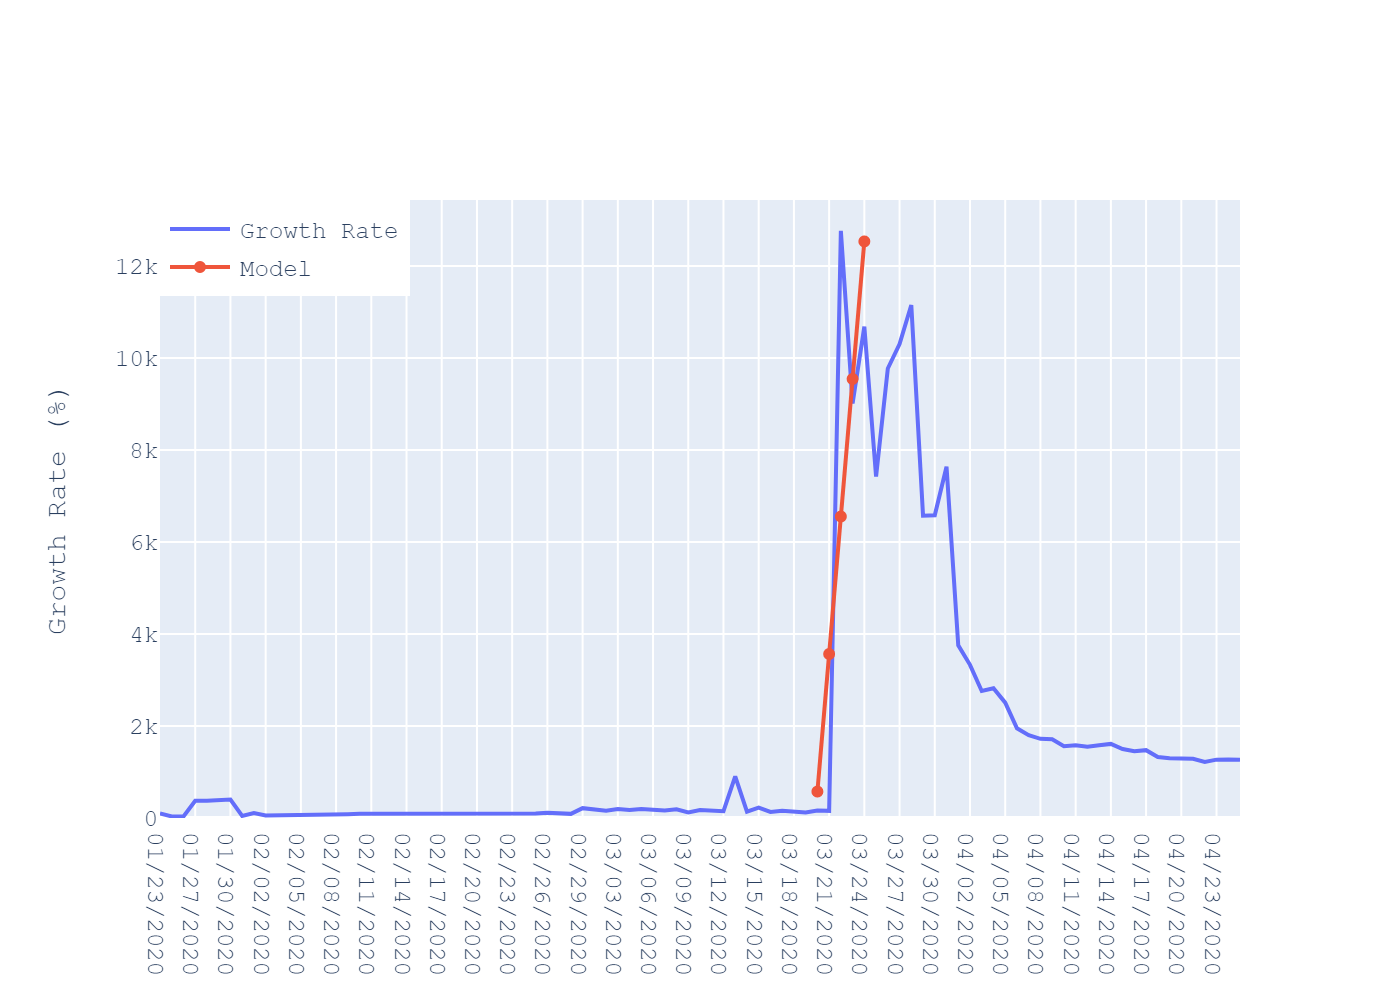
\includegraphics[scale=0.3]{task3/Australia.png}
  \caption{COVID-19 Growth Rate in Australia}
\end{figure}

\newpage
\subsubsection{Brazil}

Brazil reported its first official case of COVID-19 on February 25th. Even though the Brazilian Press Secretary tested positive for the virus on March 12th, Brazilian President Jair Bolsonaro continued to hold public parades for his supporters without wearing a mask. He has been heavily criticized for minimizing the virus and not issuing quarantines spurring regional governments and even local gangs to step up social distancing measures. After the Minister of Health, Luiz Mandetta questioned Bolsonaro's lack of measures, the President replaced him. Brazil is the current leader for COVID-19 cases in South America \cite{thebrazilianreport}.

\begin{figure}[H]
  \centering
  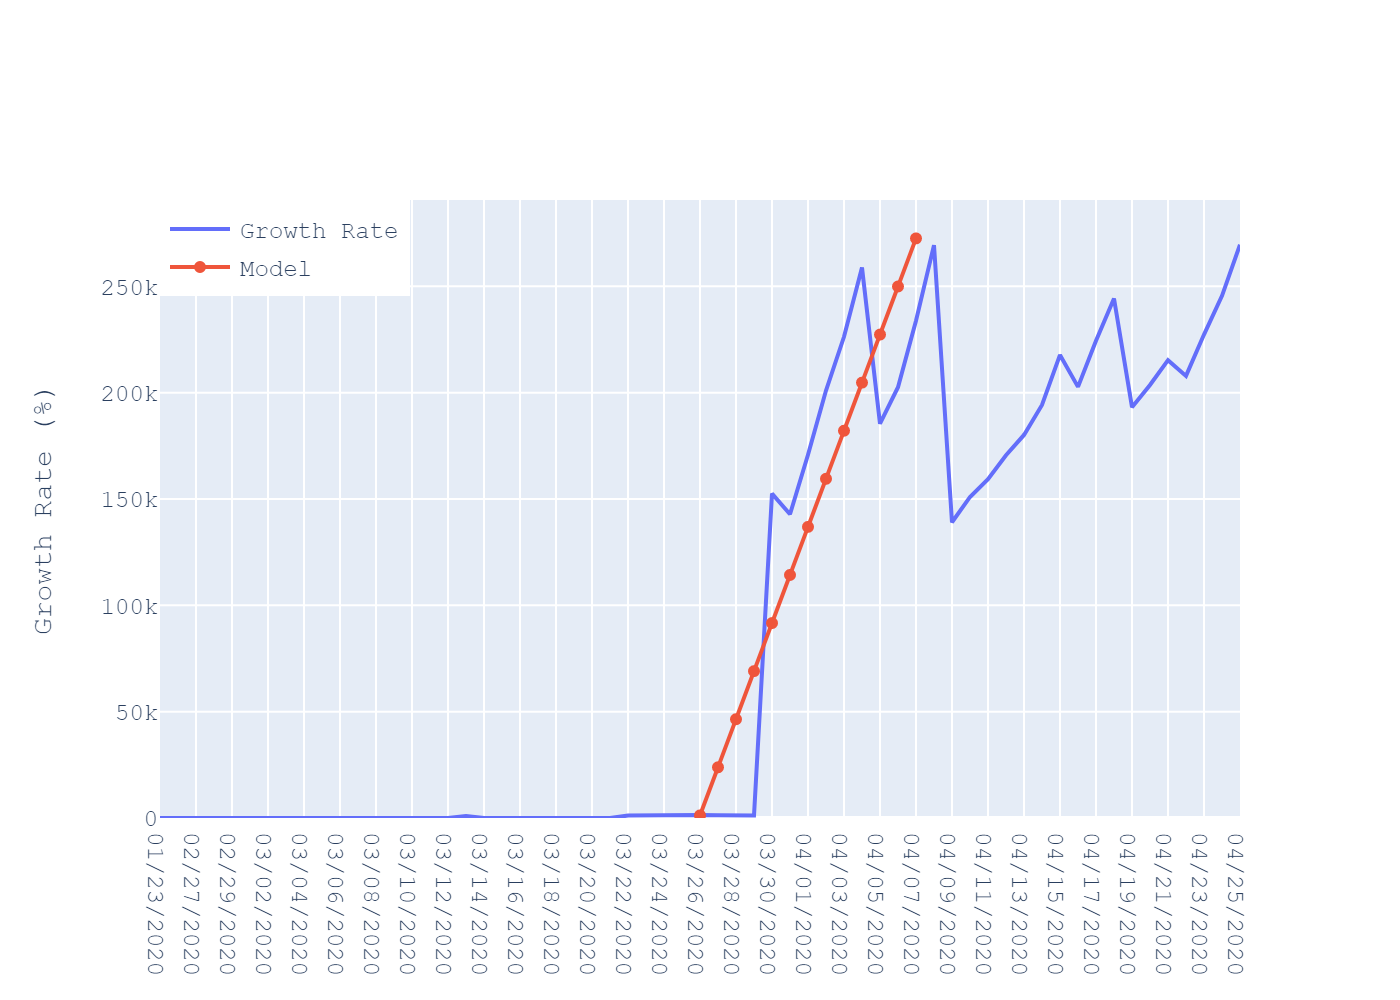
\includegraphics[scale=0.3]{task3/Brazil.png}
  \caption{COVID-19 Growth Rate in Brazil}
\end{figure}

\newpage
\subsubsection{China}

Even though reports from China state that seven cases of COVID-19 were documented in Wuhan on December 18th, 2019, Chinese scientists formally announced the new coronavirus on January 7th, 2020. On January 1th, China records its first death from COVID-19 and by January 23rd, Wuhan is placed under quarantine followed by the rest of Hubei province. An estimated 60 million residents are placed under home lockdown. China's strategy was built around testing and isolation. While a person is tested they wait in the clinic for results. If the results are positive, they are treated in the facilities until they are free of the virus and individuals who were in contact with the person are asked to self-isolate for two weeks at home. As a result of effectively removing infectious individuals from the general population, China was the first country to lower their growth rate \cite{holly_secon_2020}.

\begin{figure}[H]
  \centering
  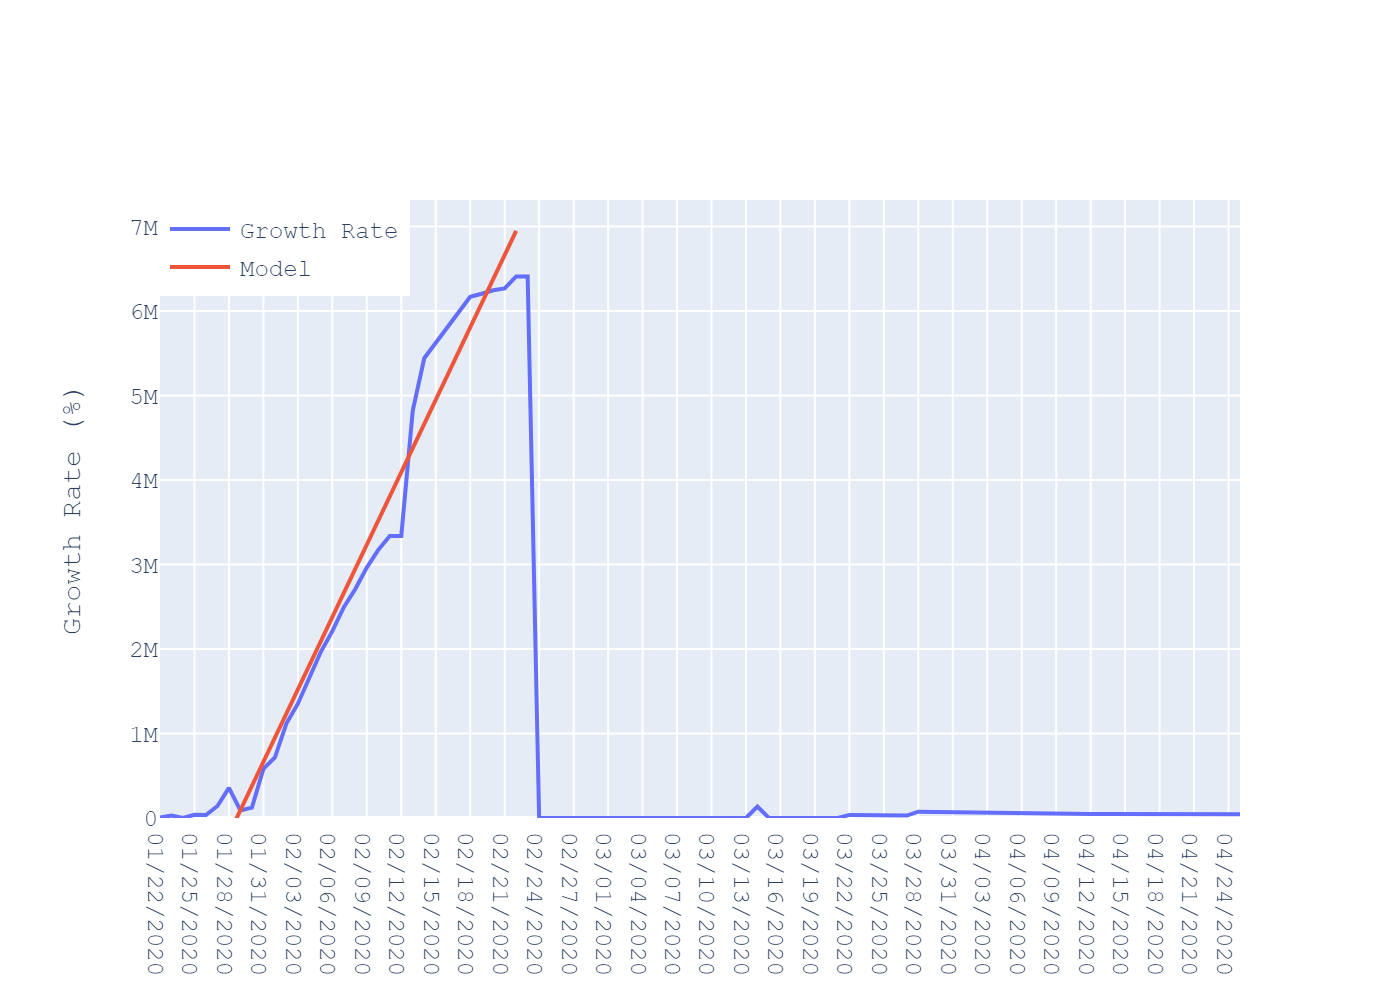
\includegraphics[scale=0.3]{task3/China.png}
  \caption{COVID-19 Growth Rate in China}
\end{figure}

\newpage
\subsubsection{South Africa}

The first case of COVID-19 in South Africa was confirmed on March 5th. On March 15th, President Cyril Ramaphosa declared a national state of disaster and imposed travel restrictions. Starting March 18th, President Ramaphosa closed schools and announced a 21-day lockdown with the deployment of the South African National Defence Force to support it. On April 9th, the lockdown was extended until the end of the month. The enforcement of the lockdown by the police and army personnel included excessive force including incidences of beatings. A byproduct of the lockdown was a lowering of crime and domestic violence associated with an alcohol banned included in the restrictions \cite{knoetze_2020}.

\begin{figure}[H]
  \centering
  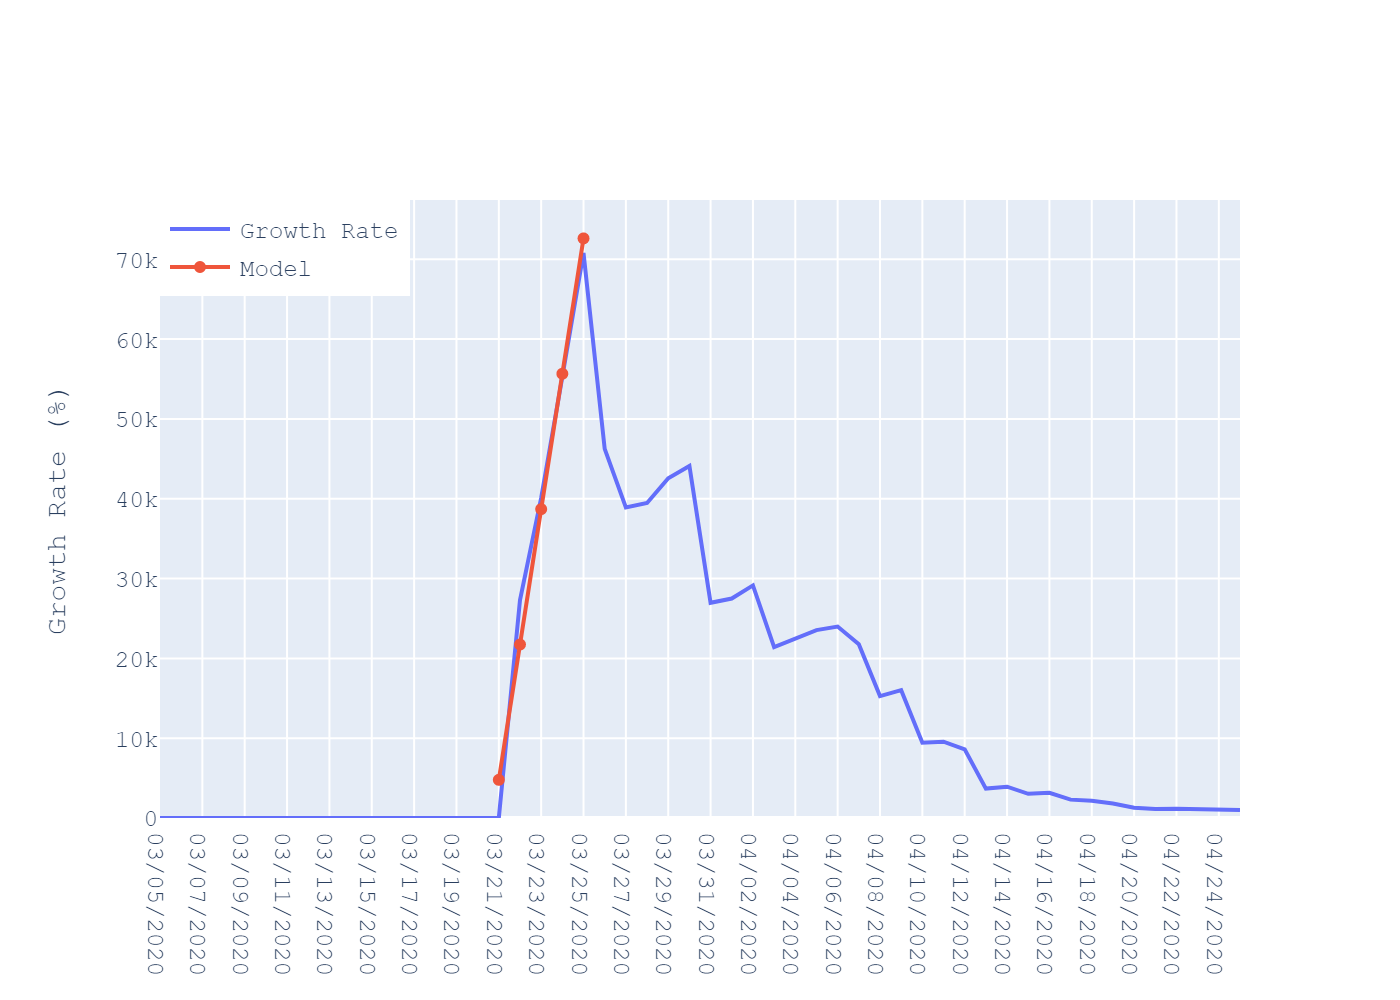
\includegraphics[scale=0.3]{task3/SouthAfrica.png}
  \caption{COVID-19 Growth Rate in South Africa}
\end{figure}

\newpage
\subsubsection{Sweden}

The first case of COVID-19 in Sweden was confirmed on January 31st. Unlike most countries, especially in Europe, Sweden has not imposed any lockdown measures. Following their constitution, the Public Health Agency can only suggest measures to the government. Currently, the agency and government have only recommended stay at home measures and social distancing but have kept schools open. The basis behind these measures are to develop a population immunity to the virus \cite{savage_2020}.

\begin{figure}[H]
  \centering
  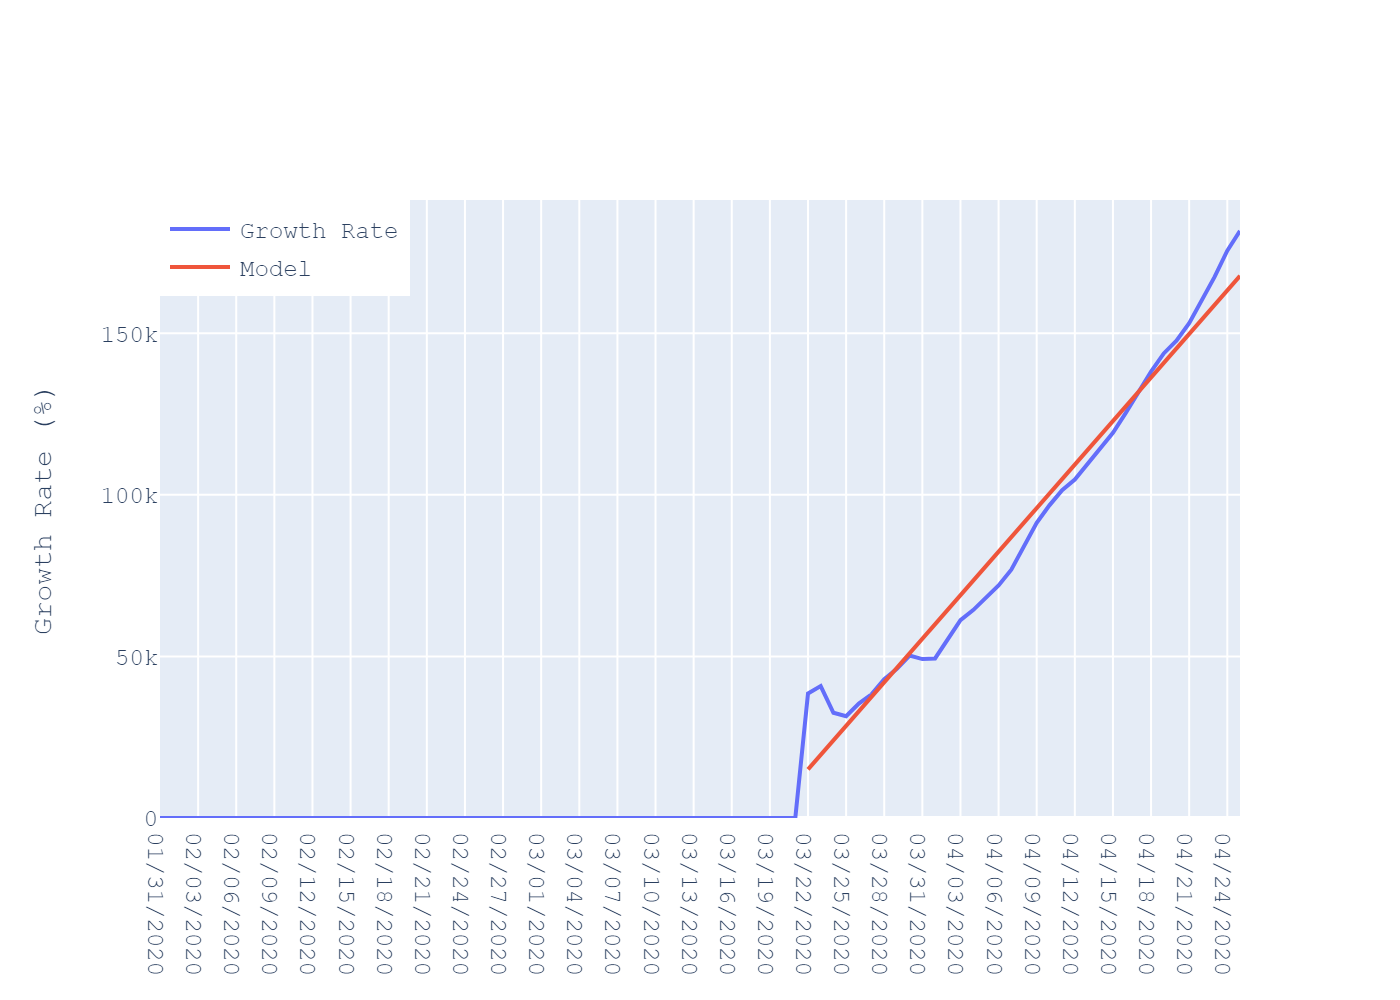
\includegraphics[scale=0.3]{task3/Sweden.png}
  \caption{COVID-19 Growth Rate in Sweden}
\end{figure}


\newpage
\subsubsection{United States}

The first confirmed case of COVID-19 was on January 20th in the state of Washington. A public health emergency was officially declared on January 31st by the Trump Administration following a ban on foreigners who recently traveled from China on February 2nd. The United States government has faced backlash for not responding the pandemic quickly, especially with a lack of testing and providing necessary medical and protective equipment. Initially President Donald Trump minimized the virus, calling it a hoax. Most efforts on containment were initiated by states like New York and California, mostly starting by March 21st. As of April 27th, states like Georgia have began easing lockdown restrictions even as the cases of COVID-19 are still climbing \cite{staff_2020}.


\begin{figure}[H]
  \centering
  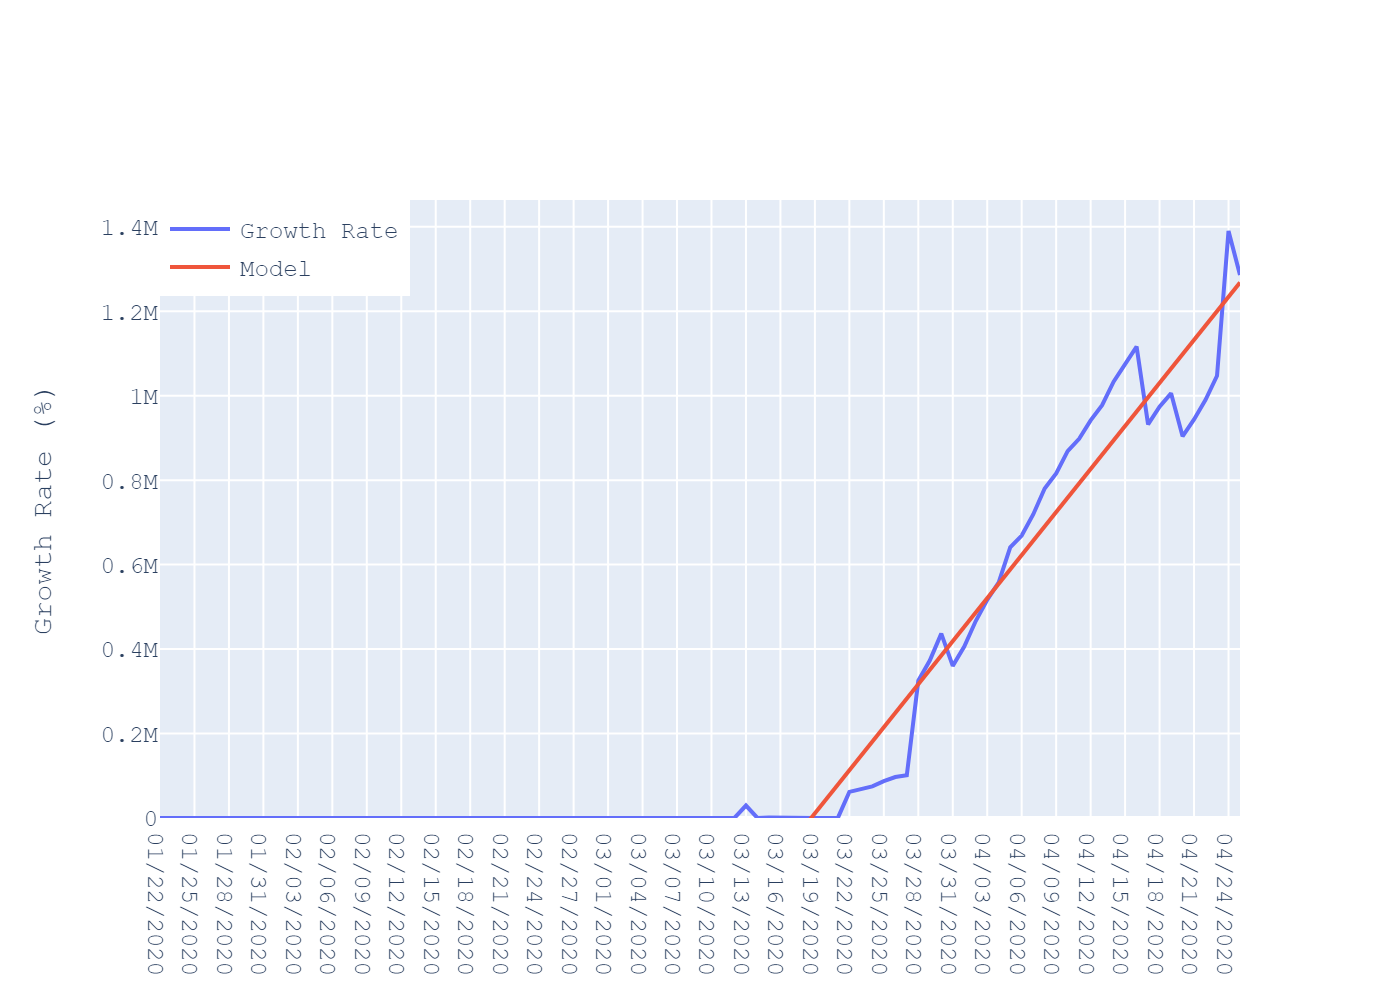
\includegraphics[scale=0.3]{task3/US.png}
  \caption{COVID-19 Growth Rate in United States}
\end{figure}

\newpage
\subsection{Results and Conclusion}

The following table summarizes the results of the growth rate analysis for the chosen countries. 

\begin{table}[H]
  \caption{COVID-19 Growth Rates and Mitigation}
  \label{Task 3 Results}
  \centering
  \begin{tabular}{llrrr}
    \toprule
    Country       & Growth Rate Slope & Start Date & End Date    & Duration \\
    \midrule
    Australia     & 2989.5            & 3/21/2020  & Continueing & 38       \\
    Brazil        & 22609.5           & 3/30/2020  & Continueing & 29       \\
    China         & 285589.4          & 1/27/2020  & 2/24/2020   & 28       \\
    South Africa  & 16959.4           & 3/22/2020  & 04/24/2020  & 33       \\
    Sweden        & 4491.7            & 3/22/2020  & Continueing & 37       \\
    United States & 33966.3           & 3/13/2020  & Continueing & 46       \\
    \bottomrule
  \end{tabular}
\end{table}

It can be seen that countries which addressed the pandemic early, like Australia and South Africa, were able to successfully mitigate the growth rate. Countries with strong governments, like China, were able to control the population in order to suppress the growth of the virus. Countries with leaders that did not address the pandemic early or at all, such as Brazil and the United States, have high growth rate numbers and not a clear end date. Countries like Sweden, who purposely do not control the population, have reasonable high growth rate but the effects on the population are still to be determined. 

\newpage
\section{Effects of Weather Conditions}
\subsection{Methodology}

In the early days of the COVID-19 spread, scientists and news establishments made assumptions that based on virus' flu-like symptoms, it would subside into the spring and summer as hot temperatures arrived in the Northern hemisphere \cite{aubrey_2020}. The National Oceanic and Atmospheric Administration, NOAA, provides free and widely available data on current and historic weather conditions for the United States. This data can be used to analyze a correlation between the virus spread and the weather conditions of the most affected states in different climates.

\begin{table}[H]
  \caption{Spread of COVID-19 in United States}
  \label{Task 4 States}
  \centering
  \begin{tabular}{lrrrrr}
    \toprule
    State         & Confirmed & Deaths & Recovered & Eradicated & Active  \\
    \midrule
    New York      & 5255780   & 292667 & 0         & 292667     & 4963113 \\
    New Jersey    & 1709925   & 71989  & 2         & 71991      & 1637934 \\
    Massachusetts & 718242    & 26601  & 8         & 26609      & 691633  \\
    California    & 673356    & 21472  & 40        & 21512      & 651844  \\
    Michigan      & 659639    & 42361  & 0         & 42361      & 617278  \\
    Pennsylvania  & 620092    & 19423  & 0         & 19423      & 600669  \\
    Illinois      & 591453    & 22091  & 16        & 22107      & 569346  \\
    Florida       & 538499    & 14018  & 0         & 14018      & 524481  \\
    Louisiana     & 517062    & 24926  & 0         & 24926      & 492136  \\
    Texas         & 376784    & 8581   & 0         & 8581       & 368203  \\
    \bottomrule
  \end{tabular}
\end{table}

New York, California, Michigan, and Louisiana were chosen as the states to analyze using their most affected cities as the target locations for the NOAA weather station data.

\newpage
\subsection{Results}
\subsubsection{New York}

The closest correlation to COVID-19 with weather data for New York is the average wind speed with about 30\%.

\begin{figure}[H]
  \centering
  \begin{subfigure}{0.45\linewidth}
    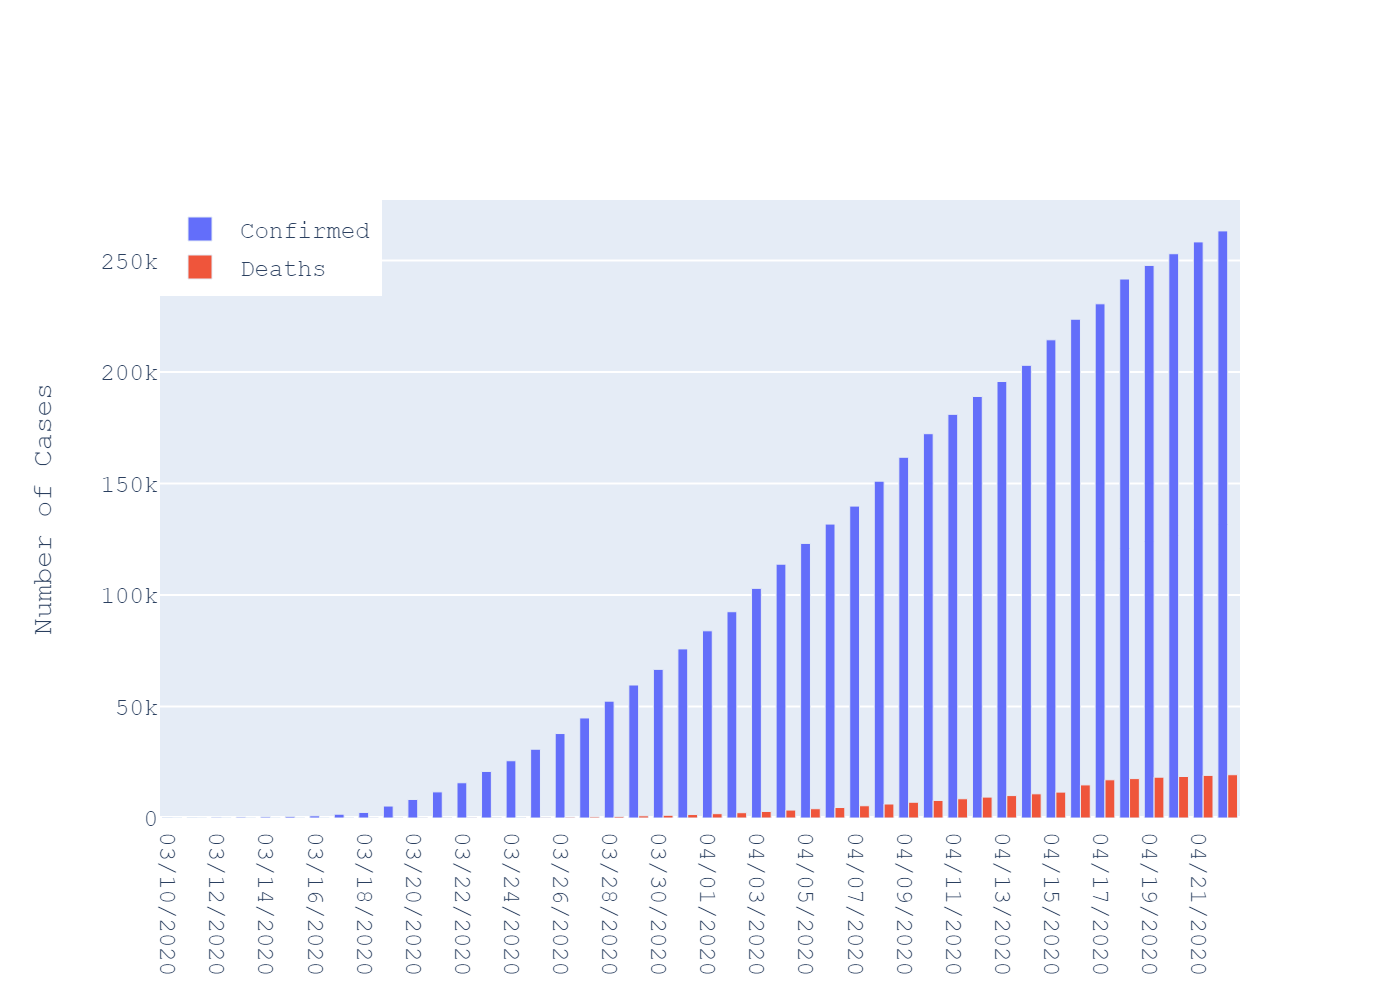
\includegraphics[width=\linewidth]{task4/New York_cases.png}
    \caption{COVID-19 Cases}
  \end{subfigure}
  \hfil
  \begin{subfigure}{0.45\linewidth}
    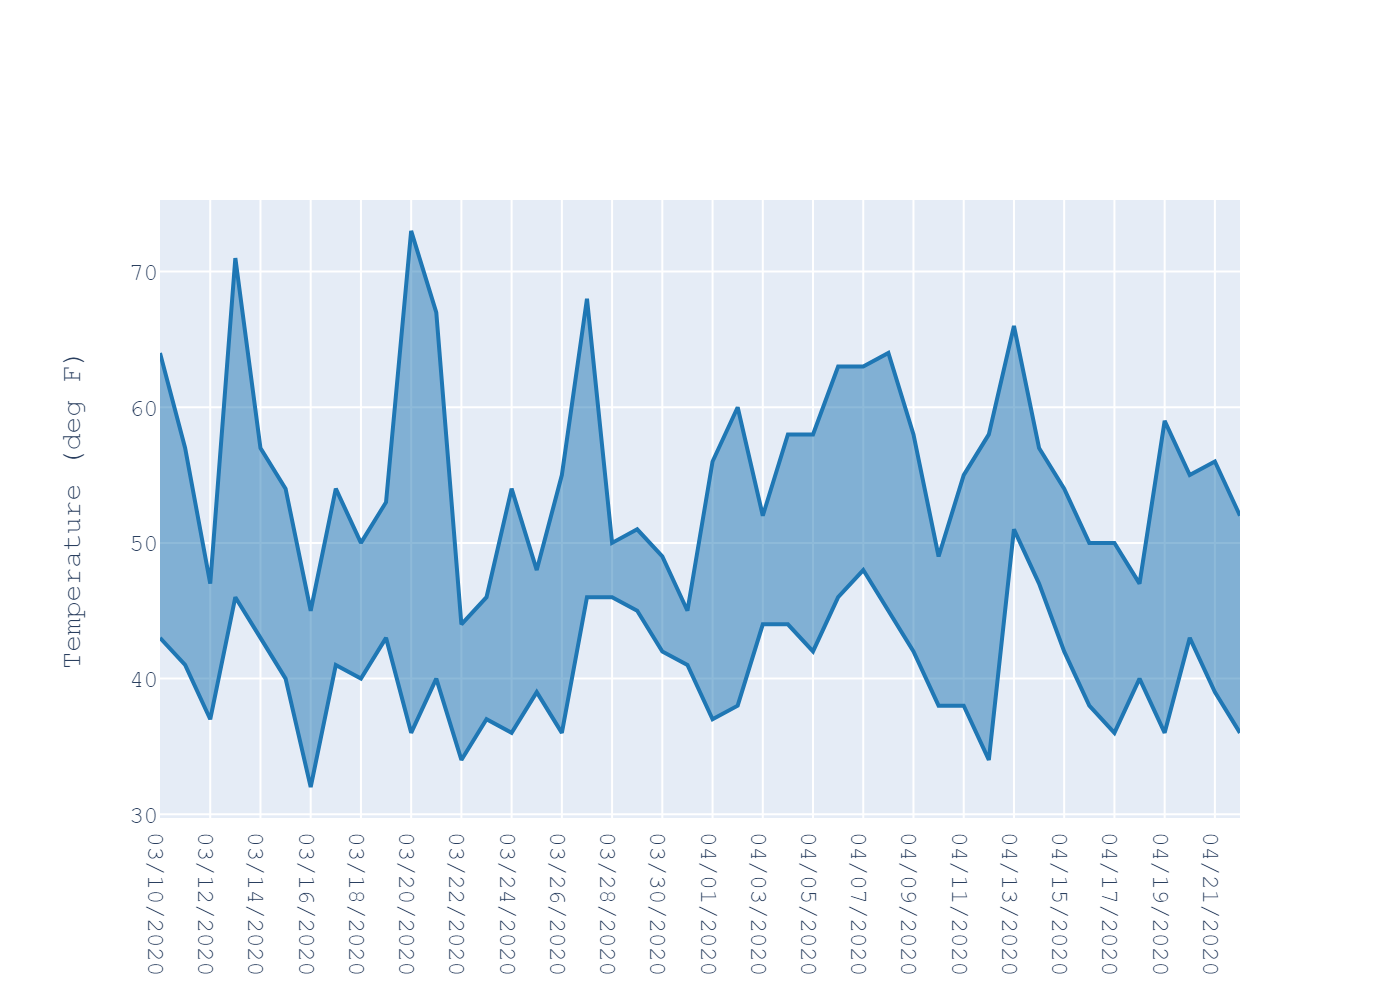
\includegraphics[width=\linewidth]{task4/New York_temp.png}
    \caption{New York City Temperature}
  \end{subfigure}

  \begin{subfigure}{0.45\linewidth}
    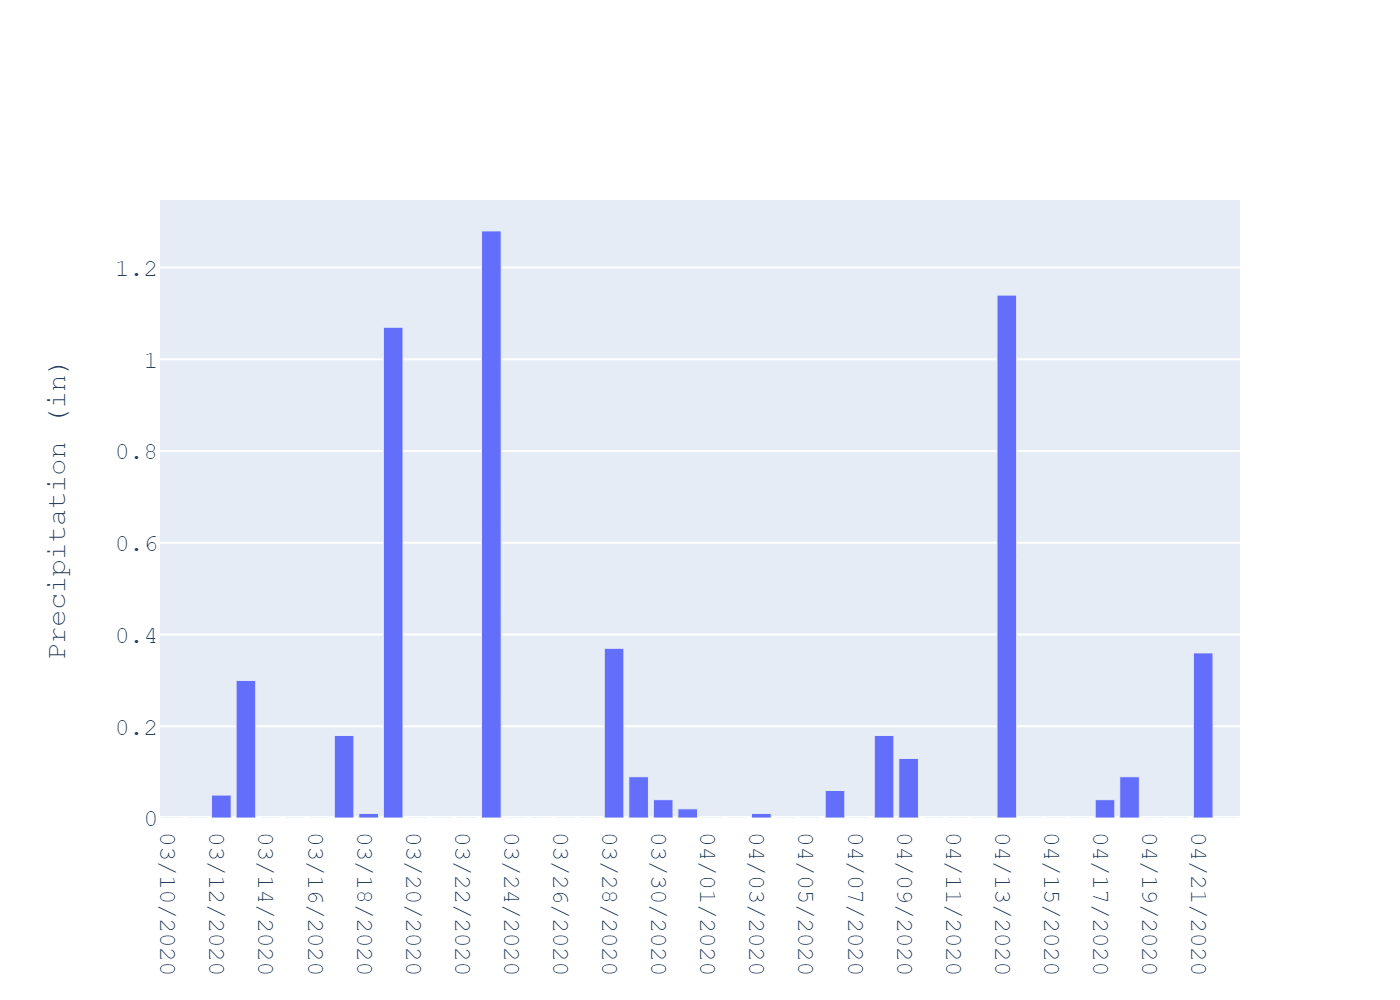
\includegraphics[width=\linewidth]{task4/New York_rain.png}
    \caption{New York City Percipitation}
  \end{subfigure}
  \hfil
  \begin{subfigure}{0.45\linewidth}
    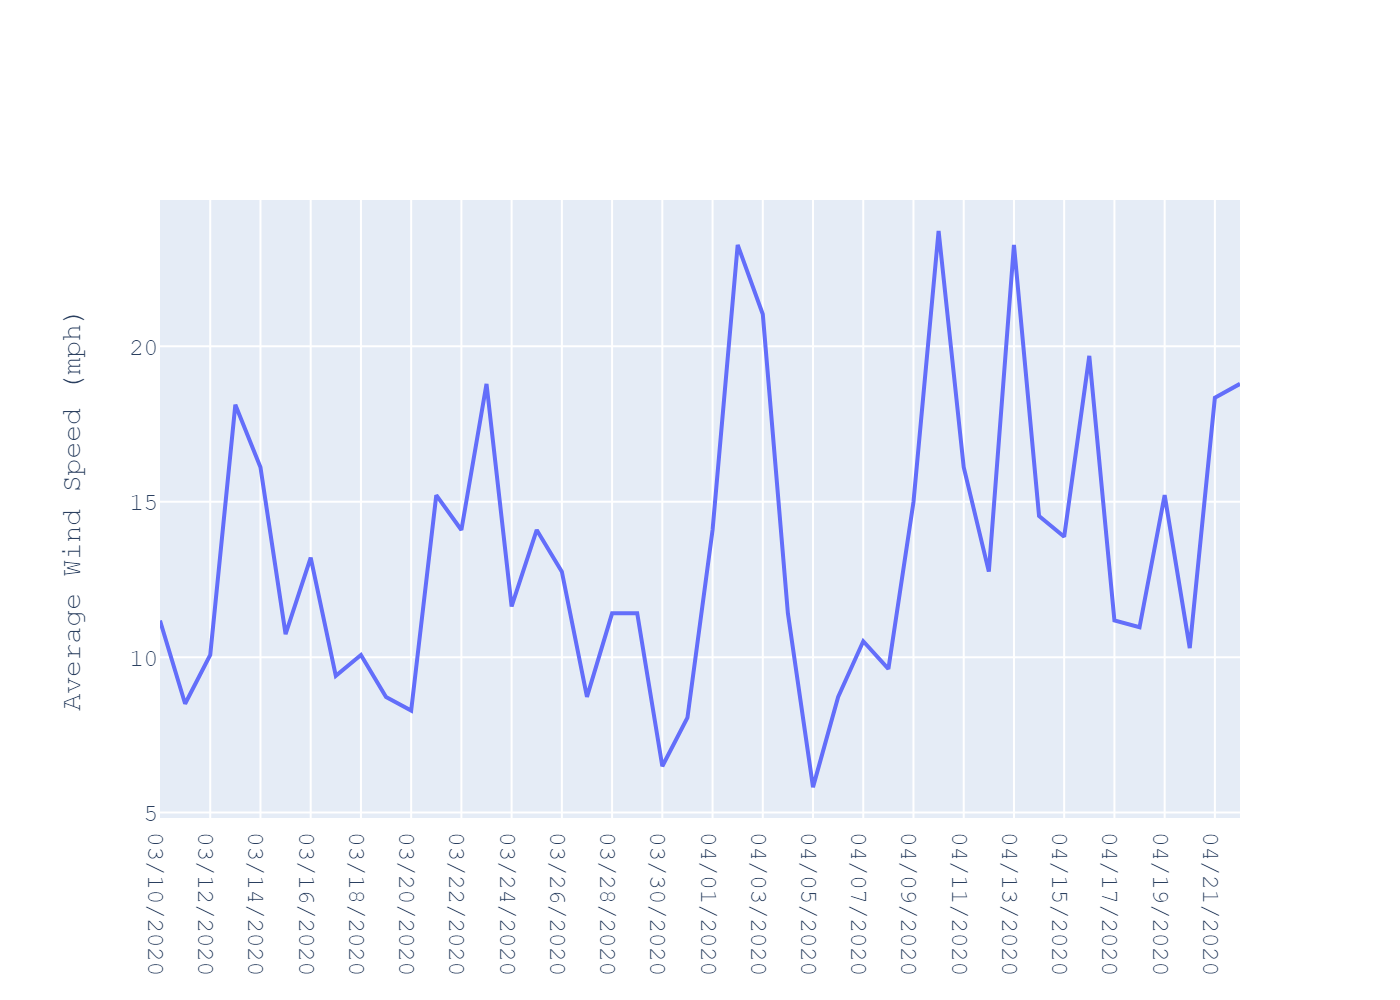
\includegraphics[width=\linewidth]{task4/New York_wnd.png}
    \caption{New York City Wind Speed}
  \end{subfigure}

  \caption{New York COVID-19 spread and weather conditions}
  \label{fig:task4NY}
\end{figure}

\begin{table}[H]
  \caption{Correlation between COVID-19 spread and weather conditions in New York}
  \label{Task 4 New York}
  \centering
  \begin{tabular}{lrrrrrr}
\toprule
{} &  Confirmed &    Deaths &      AWND &      PRCP &      TMAX &      TMIN \\
\midrule
Confirmed &   1.000000 &  0.953431 &  0.306049 & -0.067988 & -0.019127 &  0.042965 \\
Deaths    &   0.953431 &  1.000000 &  0.282089 & -0.052875 & -0.059731 & -0.069921 \\
AWND      &   0.306049 &  0.282089 &  1.000000 &  0.232747 & -0.009109 & -0.086285 \\
PRCP      &  -0.067988 & -0.052875 &  0.232747 &  1.000000 & -0.004461 &  0.257297 \\
TMAX      &  -0.019127 & -0.059731 & -0.009109 & -0.004461 &  1.000000 &  0.431357 \\
TMIN      &   0.042965 & -0.069921 & -0.086285 &  0.257297 &  0.431357 &  1.000000 \\
\bottomrule
\end{tabular}

\end{table}


\newpage
\subsubsection{California}

The closest correlation to COVID-19 with weather data for California is the daily lower temperature with about 35\%.

\begin{figure}[H]
  \centering
  \begin{subfigure}{0.45\linewidth}
    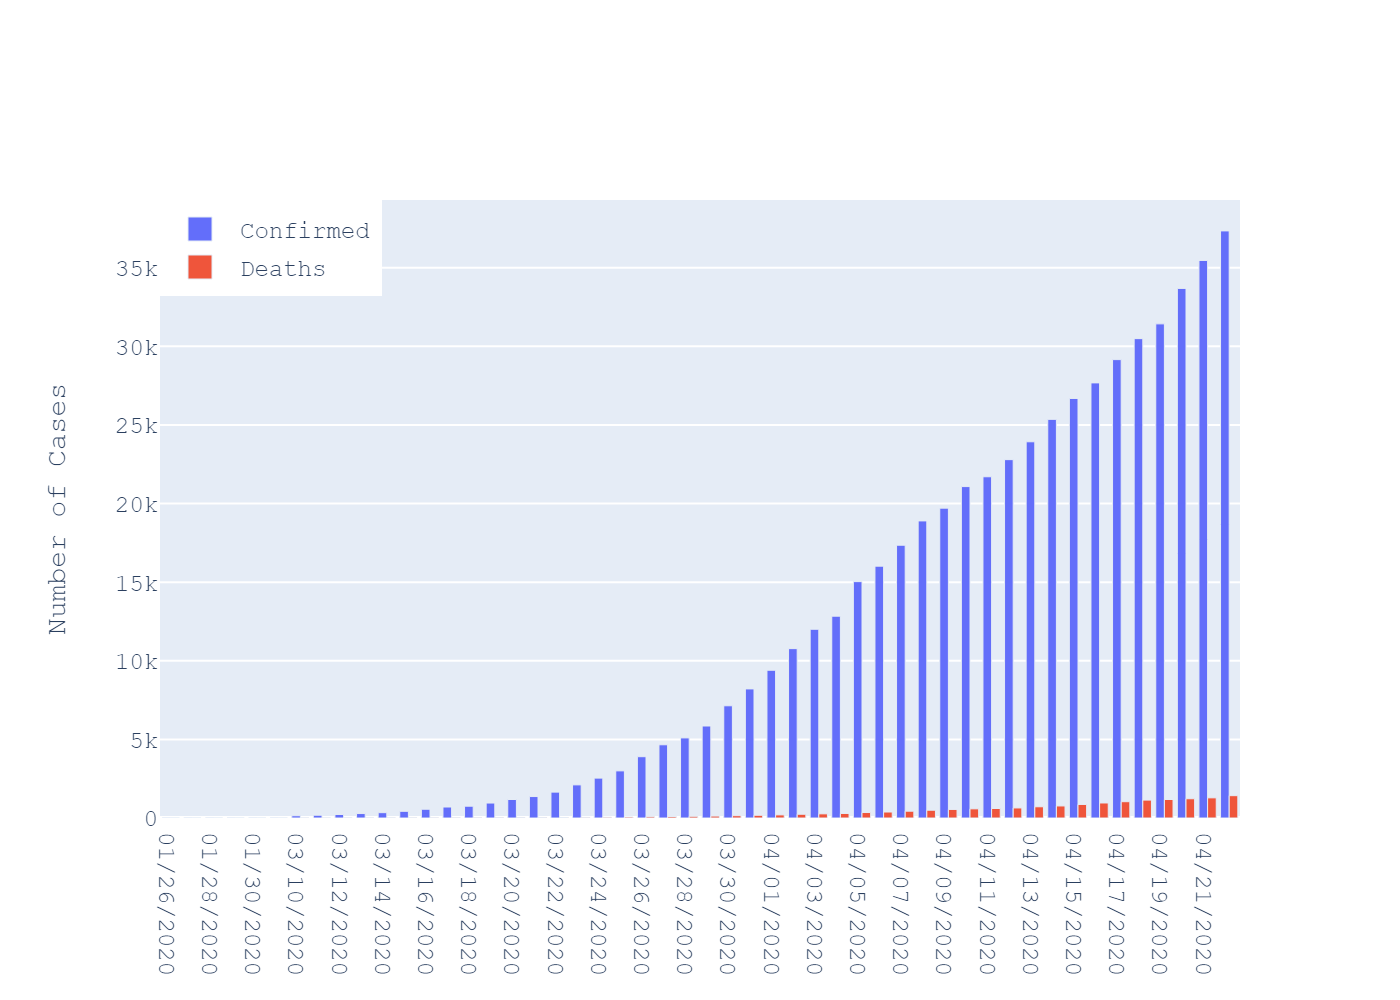
\includegraphics[width=\linewidth]{task4/California_cases.png}
    \caption{California COVID-19 Cases}
  \end{subfigure}
  \hfil
  \begin{subfigure}{0.45\linewidth}
    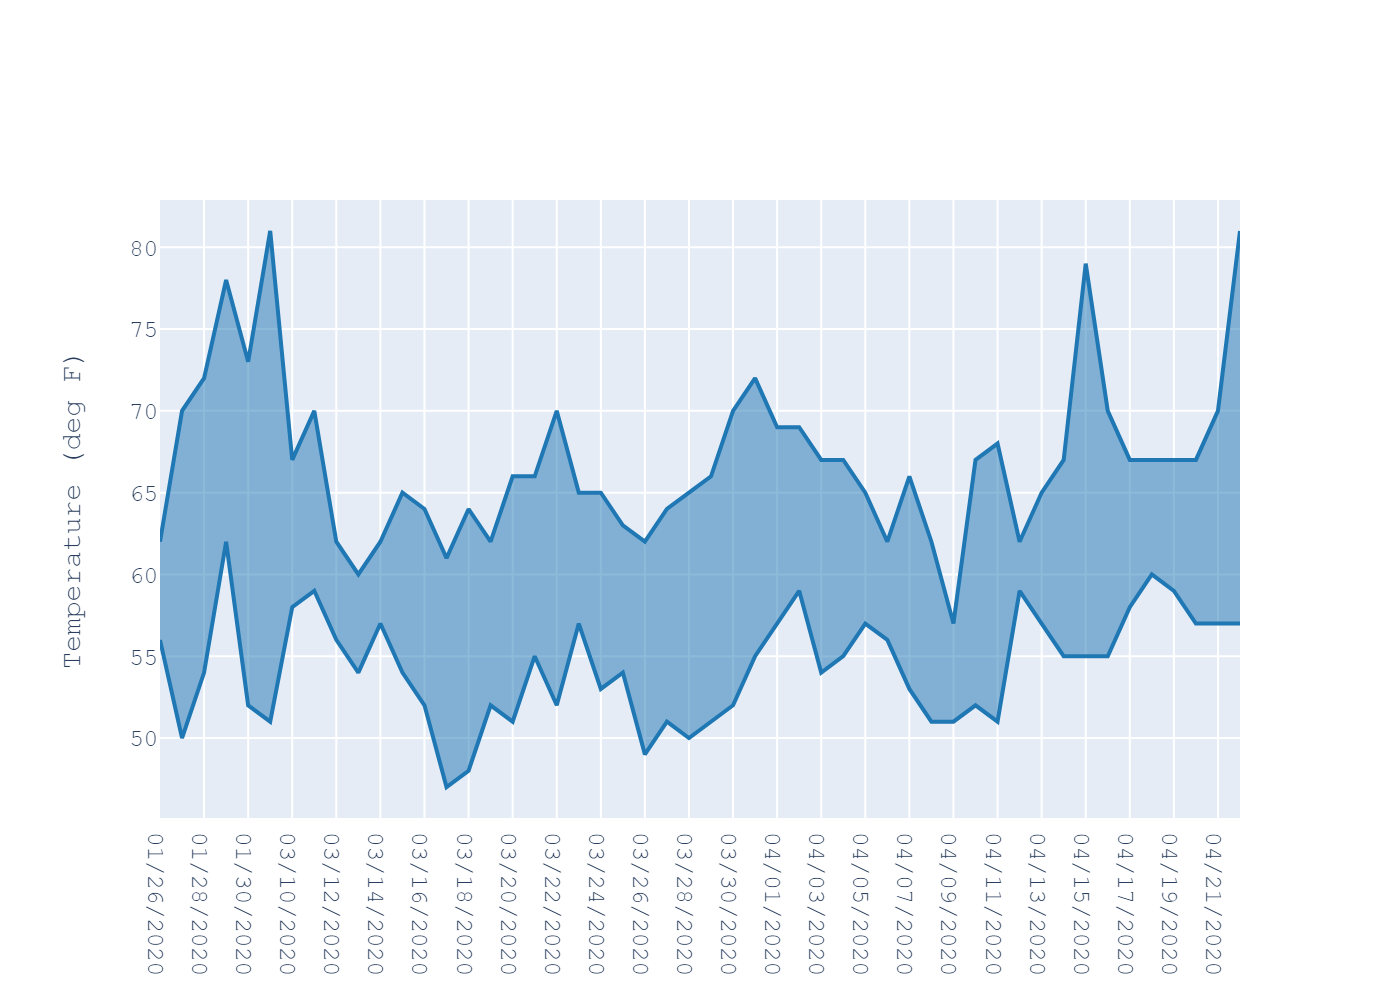
\includegraphics[width=\linewidth]{task4/California_temp.png}
    \caption{Los Angeles Temperature}
  \end{subfigure}

  \begin{subfigure}{0.45\linewidth}
    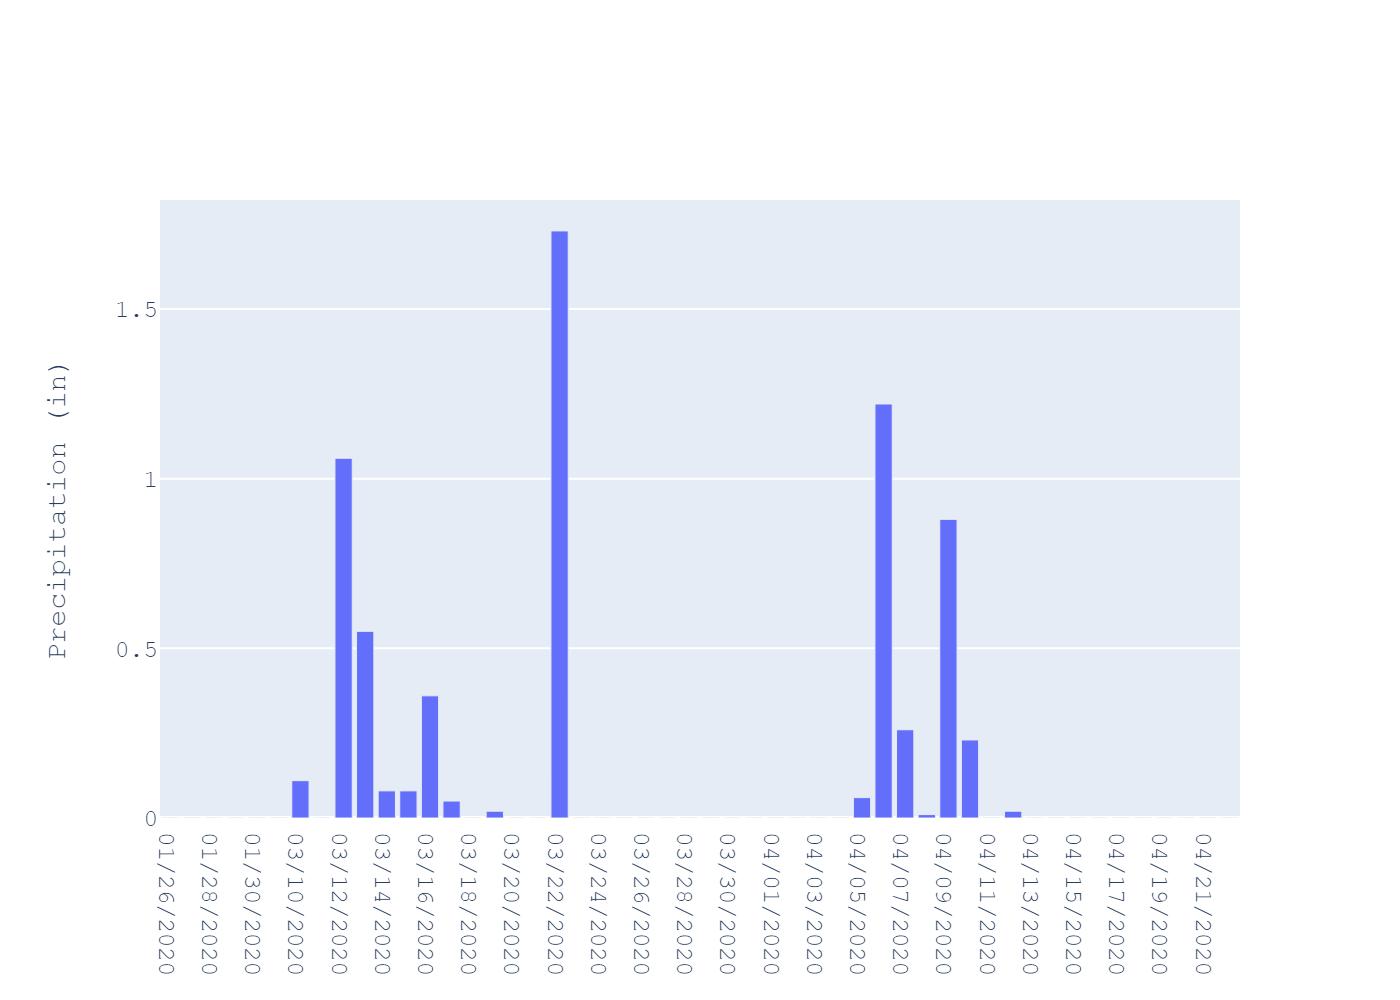
\includegraphics[width=\linewidth]{task4/California_rain.png}
    \caption{Los Angeles Percipitation}
  \end{subfigure}
  \hfil
  \begin{subfigure}{0.45\linewidth}
    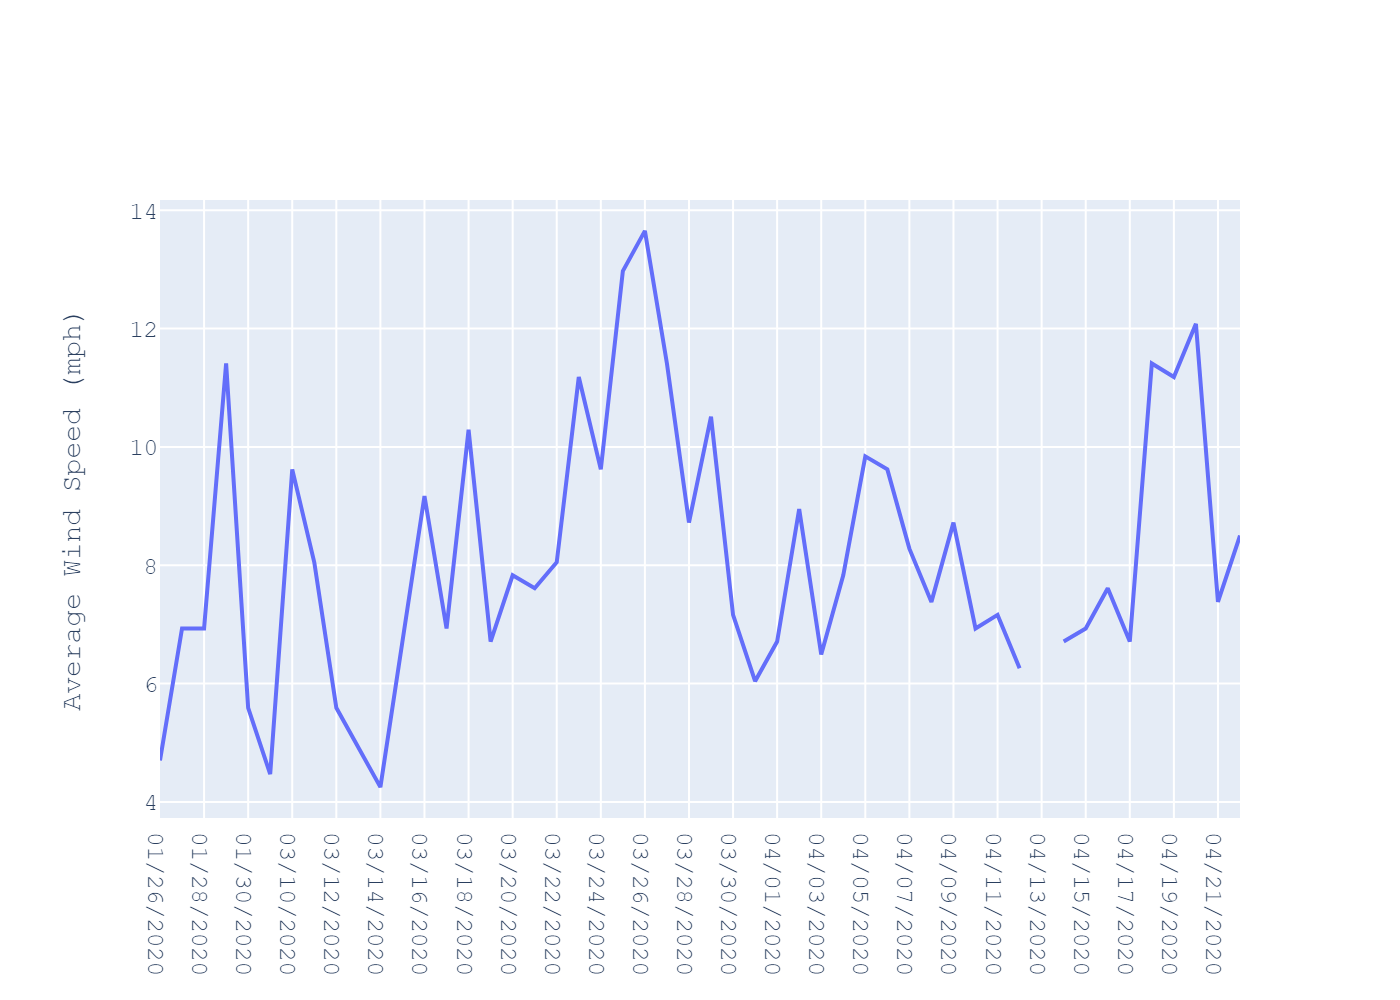
\includegraphics[width=\linewidth]{task4/California_wnd.png}
    \caption{Los Angeles Wind Speed}
  \end{subfigure}

  \caption{California COVID-19 spread and weather conditions}
  \label{fig:task4CA}
\end{figure}

\begin{table}[H]
  \caption{Correlation between COVID-19 spread and weather conditions in California}
  \label{Task 4 California}
  \centering
  \begin{tabular}{lrrrrrr}
\toprule
{} &  Confirmed &    Deaths &      AWND &      PRCP &      TMAX &      TMIN \\
\midrule
Confirmed &   1.000000 &  0.983698 &  0.126789 & -0.110202 &  0.173194 &  0.358537 \\
Deaths    &   0.983698 &  1.000000 &  0.141337 & -0.130792 &  0.221446 &  0.385531 \\
AWND      &   0.126789 &  0.141337 &  1.000000 & -0.068453 & -0.113743 &  0.074694 \\
PRCP      &  -0.110202 & -0.130792 & -0.068453 &  1.000000 & -0.241972 & -0.082043 \\
TMAX      &   0.173194 &  0.221446 & -0.113743 & -0.241972 &  1.000000 &  0.231867 \\
TMIN      &   0.358537 &  0.385531 &  0.074694 & -0.082043 &  0.231867 &  1.000000 \\
\bottomrule
\end{tabular}

\end{table}

\newpage
\subsubsection{Michigan}

The closest correlation to COVID-19 with weather data for Michigan are the daily high and low temperatures with approximately 40\% and 39\%, respectively.

\begin{figure}[H]
  \centering
  \begin{subfigure}{0.45\linewidth}
    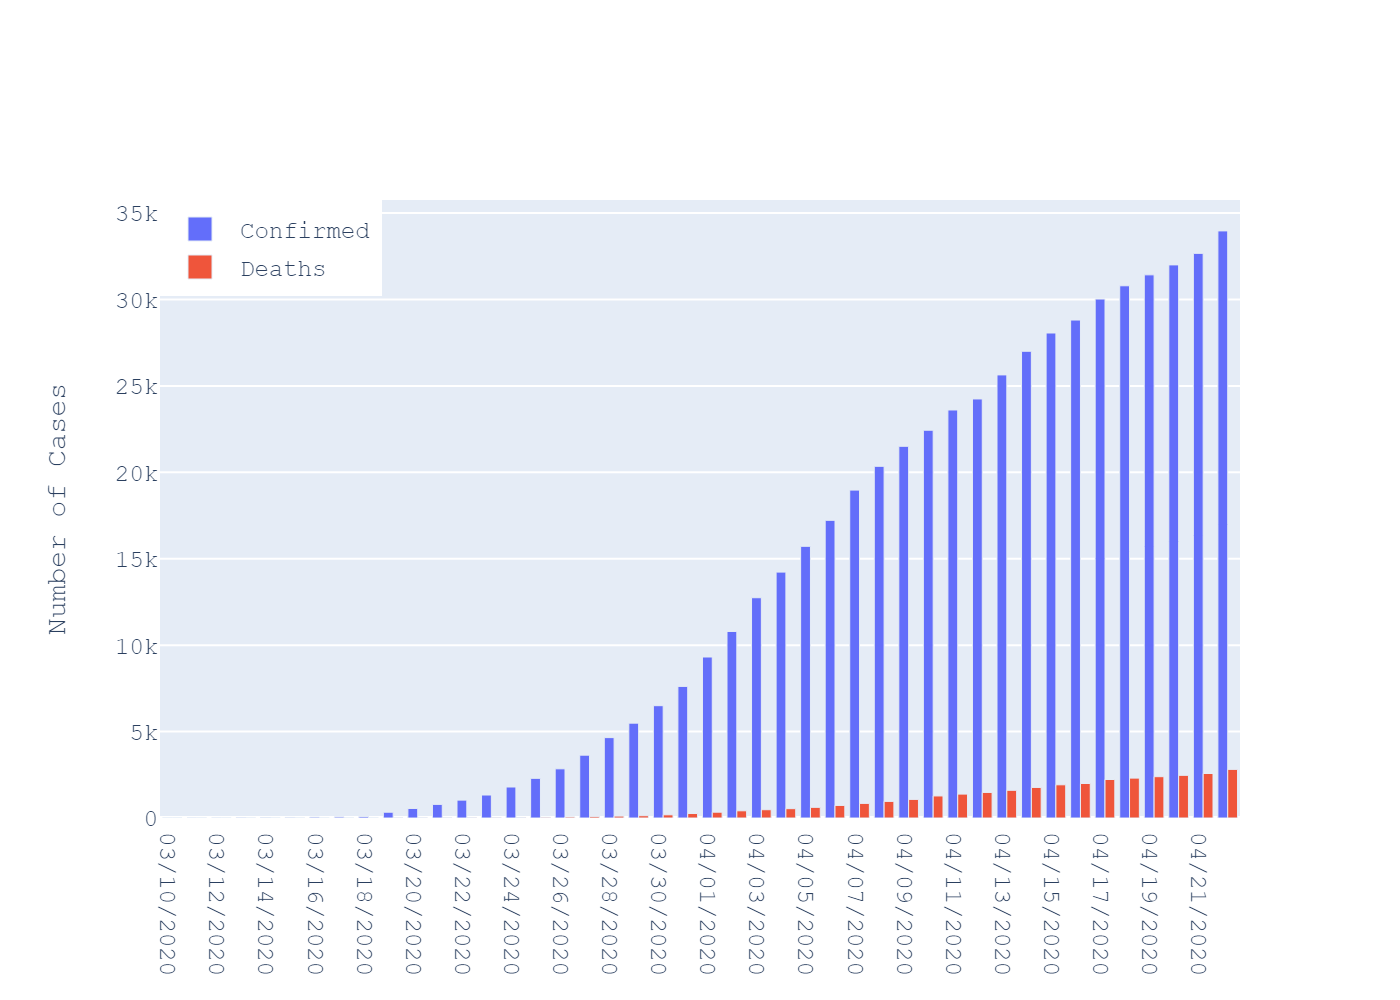
\includegraphics[width=\linewidth]{task4/Michigan_cases.png}
    \caption{Michigan COVID-19 Cases}
  \end{subfigure}
  \hfil
  \begin{subfigure}{0.45\linewidth}
    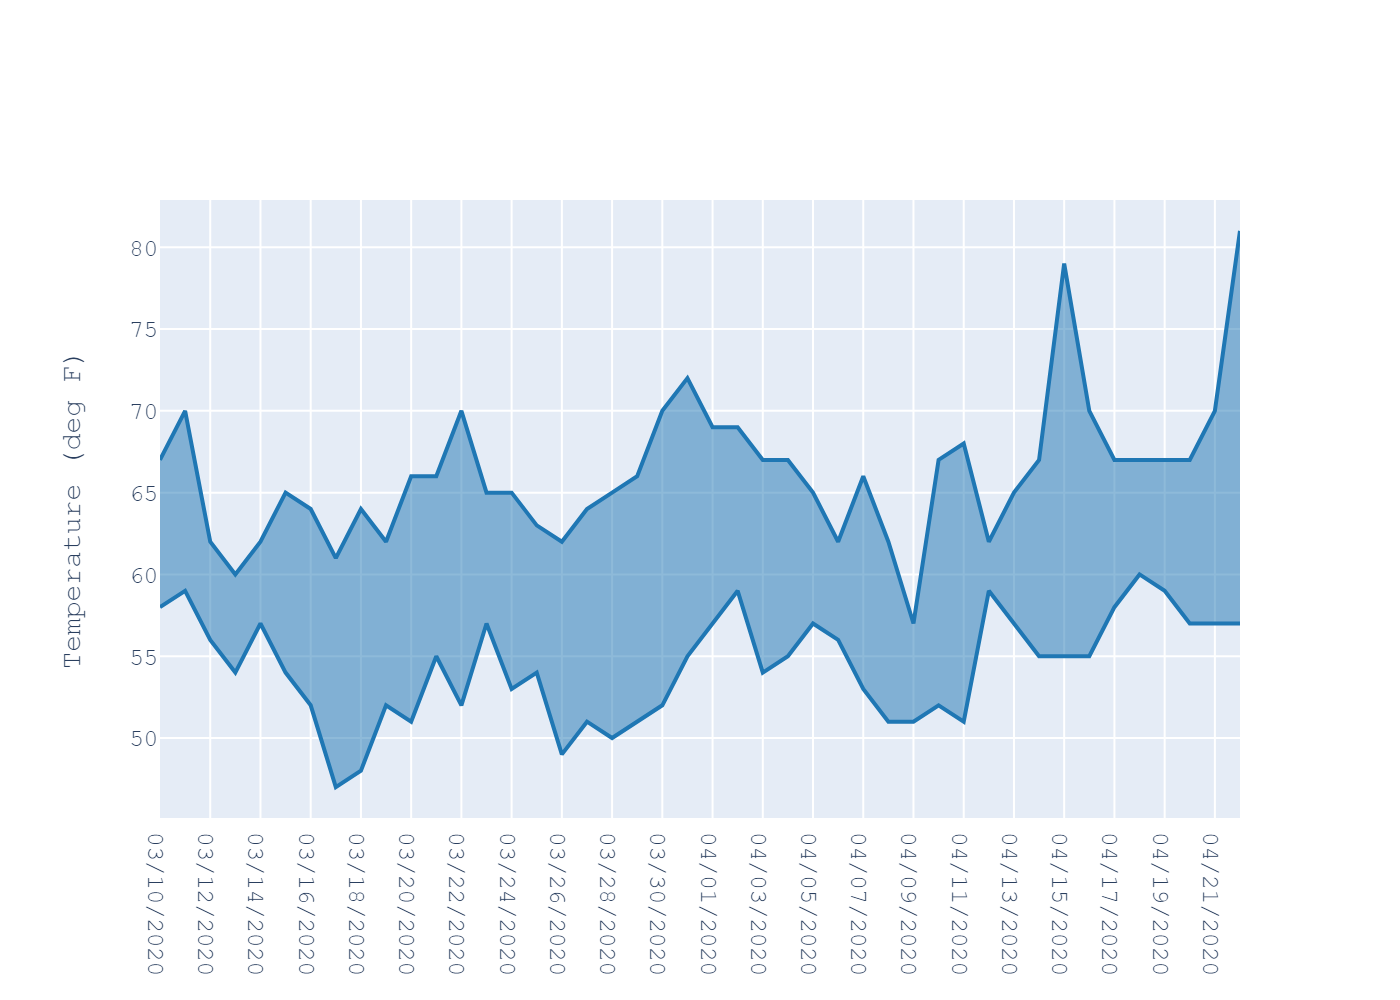
\includegraphics[width=\linewidth]{task4/Michigan_temp.png}
    \caption{Detroit Temperature}
  \end{subfigure}

  \begin{subfigure}{0.45\linewidth}
    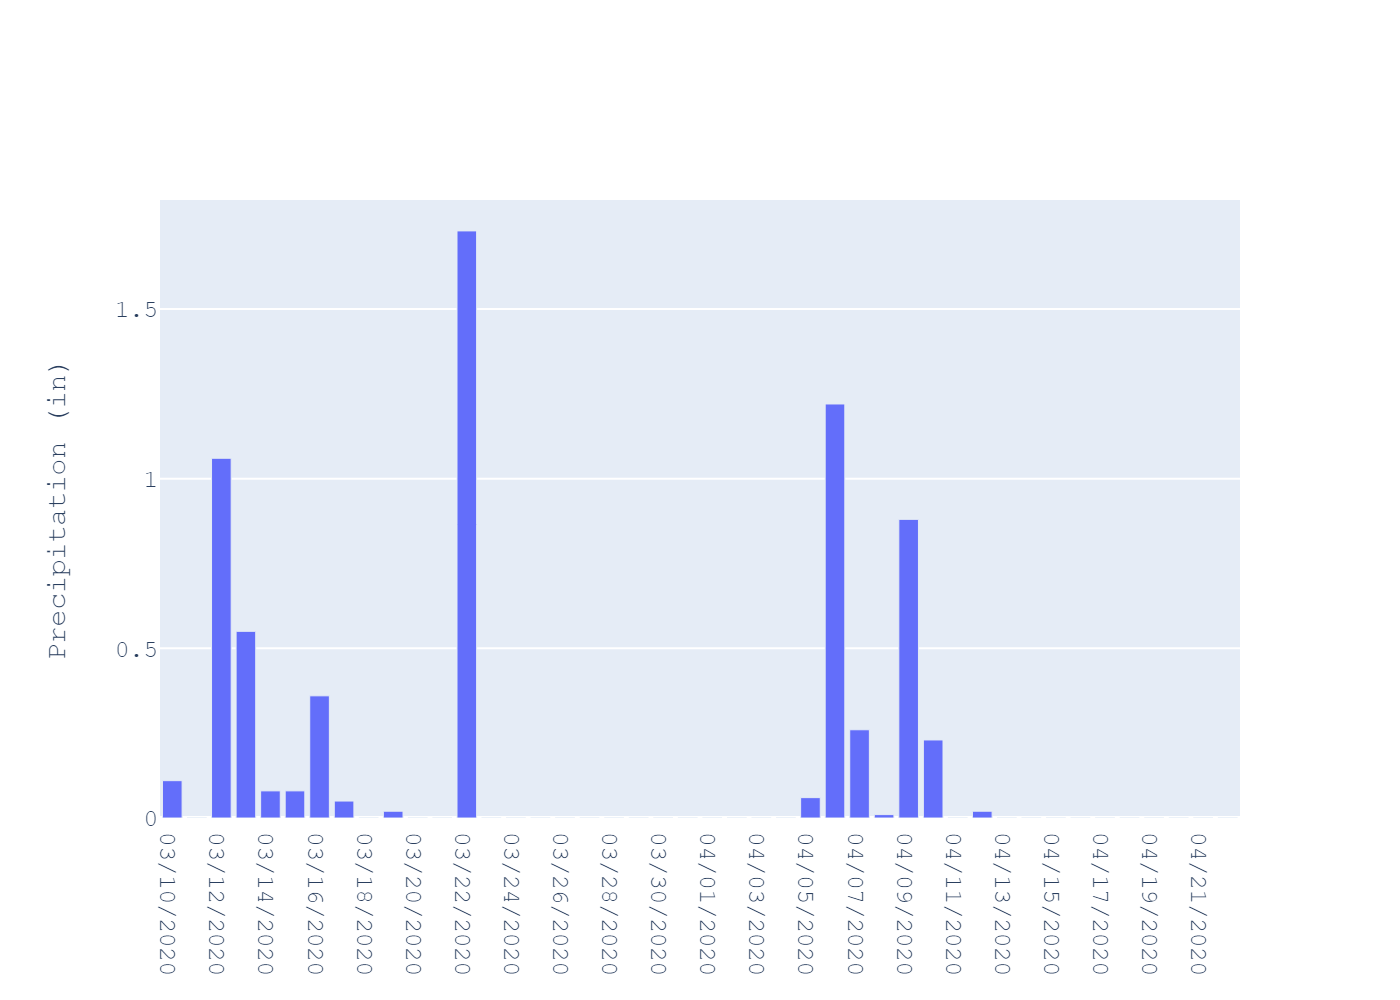
\includegraphics[width=\linewidth]{task4/Michigan_rain.png}
    \caption{Detroit Percipitation}
  \end{subfigure}
  \hfil
  \begin{subfigure}{0.45\linewidth}
    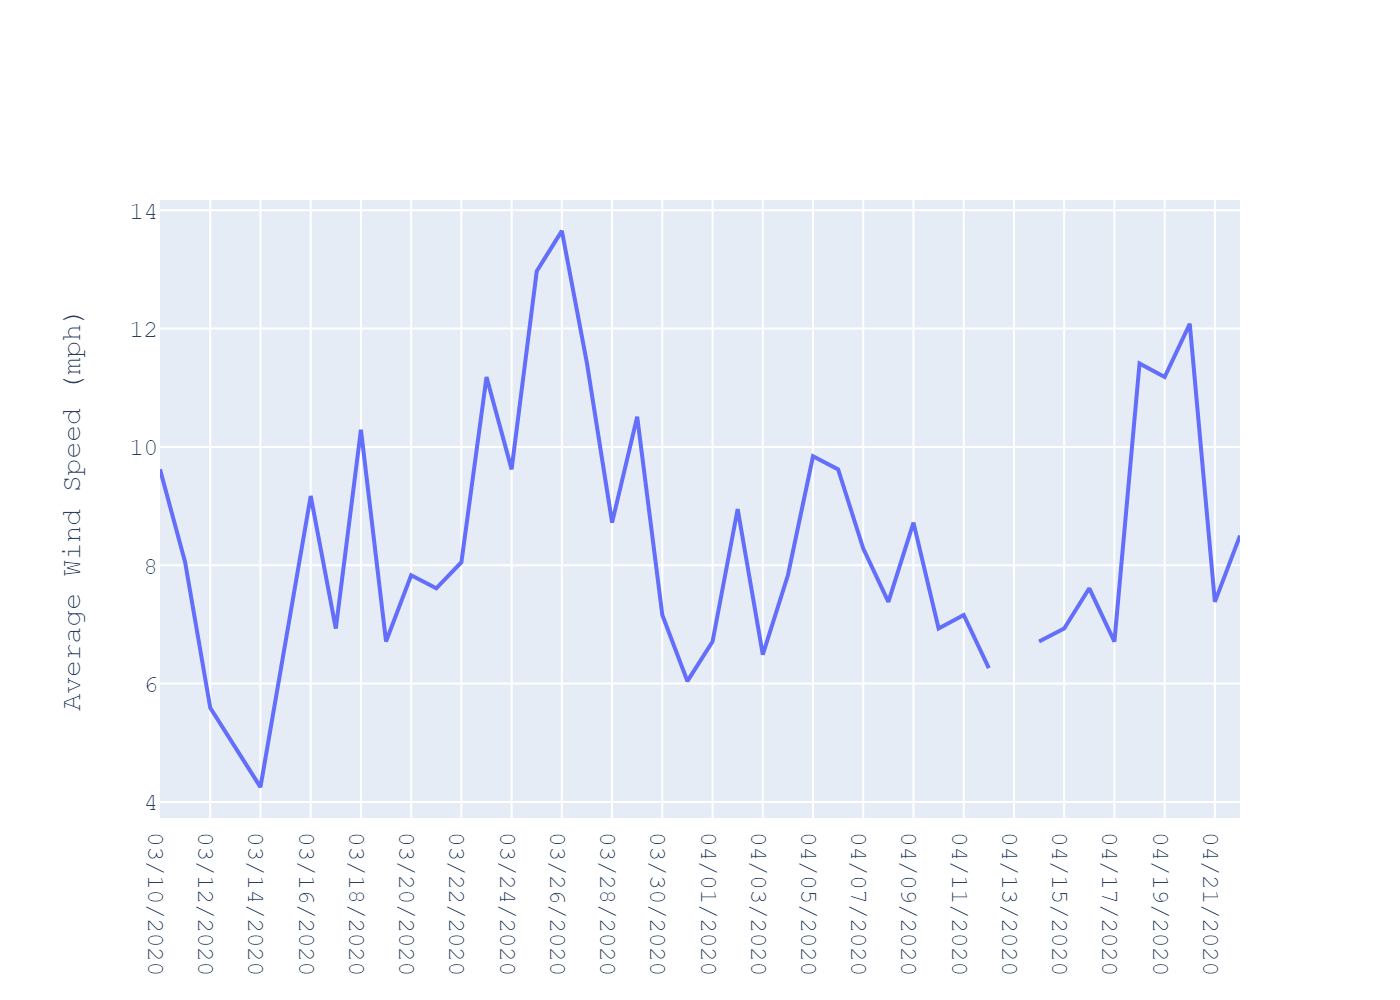
\includegraphics[width=\linewidth]{task4/Michigan_wnd.png}
    \caption{Detroit Wind Speed}
  \end{subfigure}

  \caption{Michigan COVID-19 spread and weather conditions}
  \label{fig:task4CA}
\end{figure}

\begin{table}[H]
  \caption{Correlation between COVID-19 spread and weather conditions in Michigan}
  \label{Task 4 Michigan}
  \centering
  \begin{tabular}{lrrrrrr}
\toprule
{} &  Confirmed &    Deaths &      AWND &      PRCP &      TMAX &      TMIN \\
\midrule
Confirmed &   1.000000 &  0.971463 &  0.022642 & -0.157289 &  0.387537 &  0.406781 \\
Deaths    &   0.971463 &  1.000000 &  0.041239 & -0.180878 &  0.439628 &  0.442325 \\
AWND      &   0.022642 &  0.041239 &  1.000000 & -0.118884 & -0.079533 & -0.055577 \\
PRCP      &  -0.157289 & -0.180878 & -0.118884 &  1.000000 & -0.228251 & -0.094460 \\
TMAX      &   0.387537 &  0.439628 & -0.079533 & -0.228251 &  1.000000 &  0.317699 \\
TMIN      &   0.406781 &  0.442325 & -0.055577 & -0.094460 &  0.317699 &  1.000000 \\
\bottomrule
\end{tabular}

\end{table}

\newpage
\subsubsection{Louisiana}

The closest correlation to COVID-19 with weather data for Louisiana is the daily high and lower temperatures with approximately 35\% and 40\%, respectively.

\begin{figure}[H]
  \centering
  \begin{subfigure}{0.45\linewidth}
    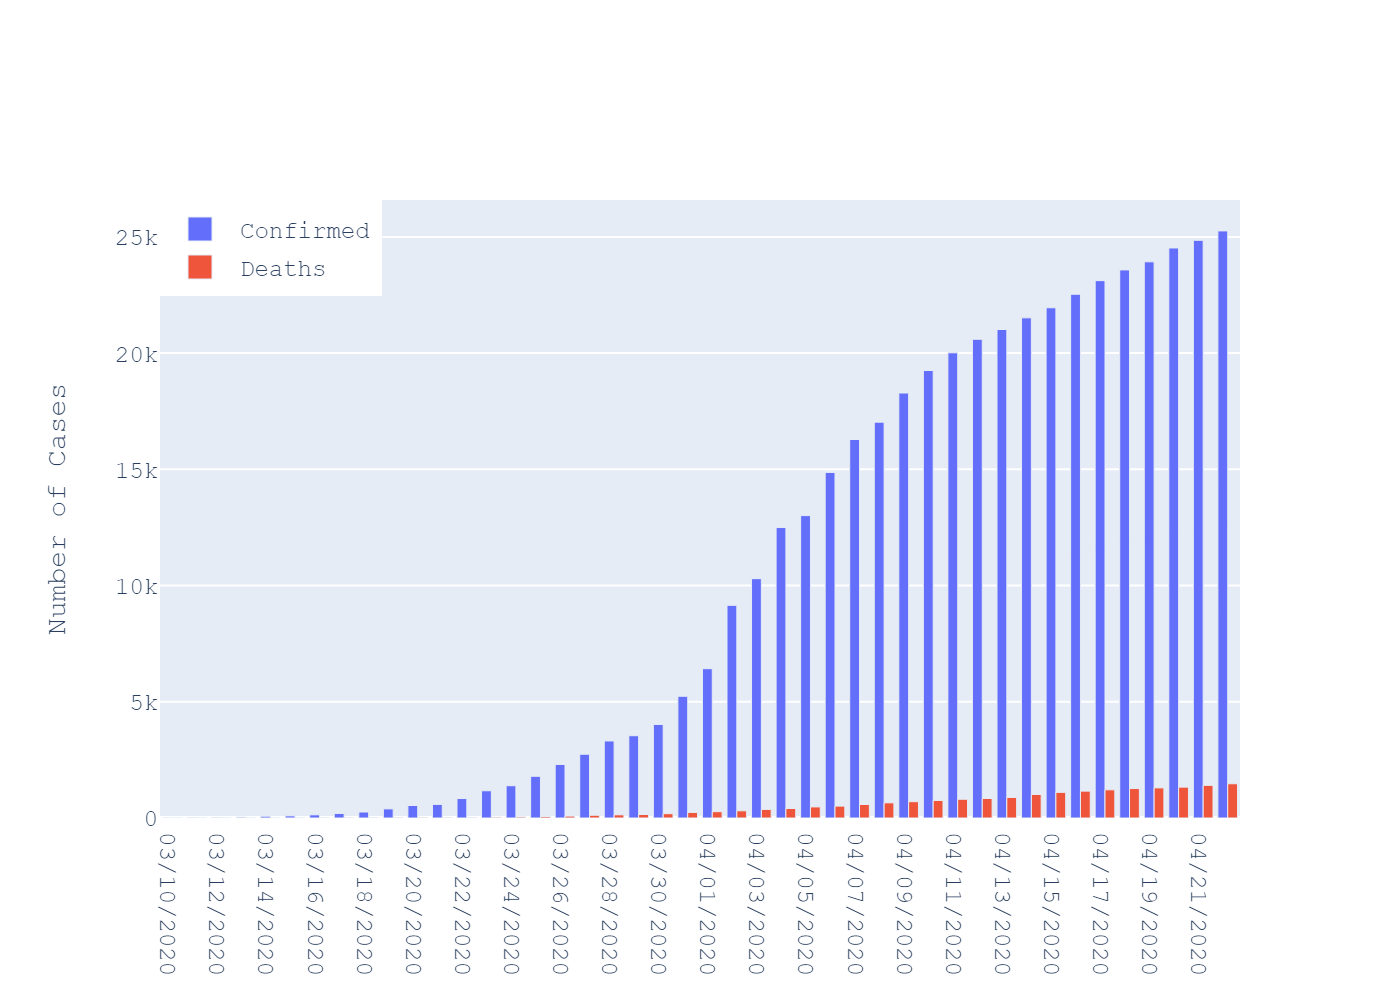
\includegraphics[width=\linewidth]{task4/Louisiana_cases.png}
    \caption{Louisiana COVID-19 Cases}
  \end{subfigure}
  \hfil
  \begin{subfigure}{0.45\linewidth}
    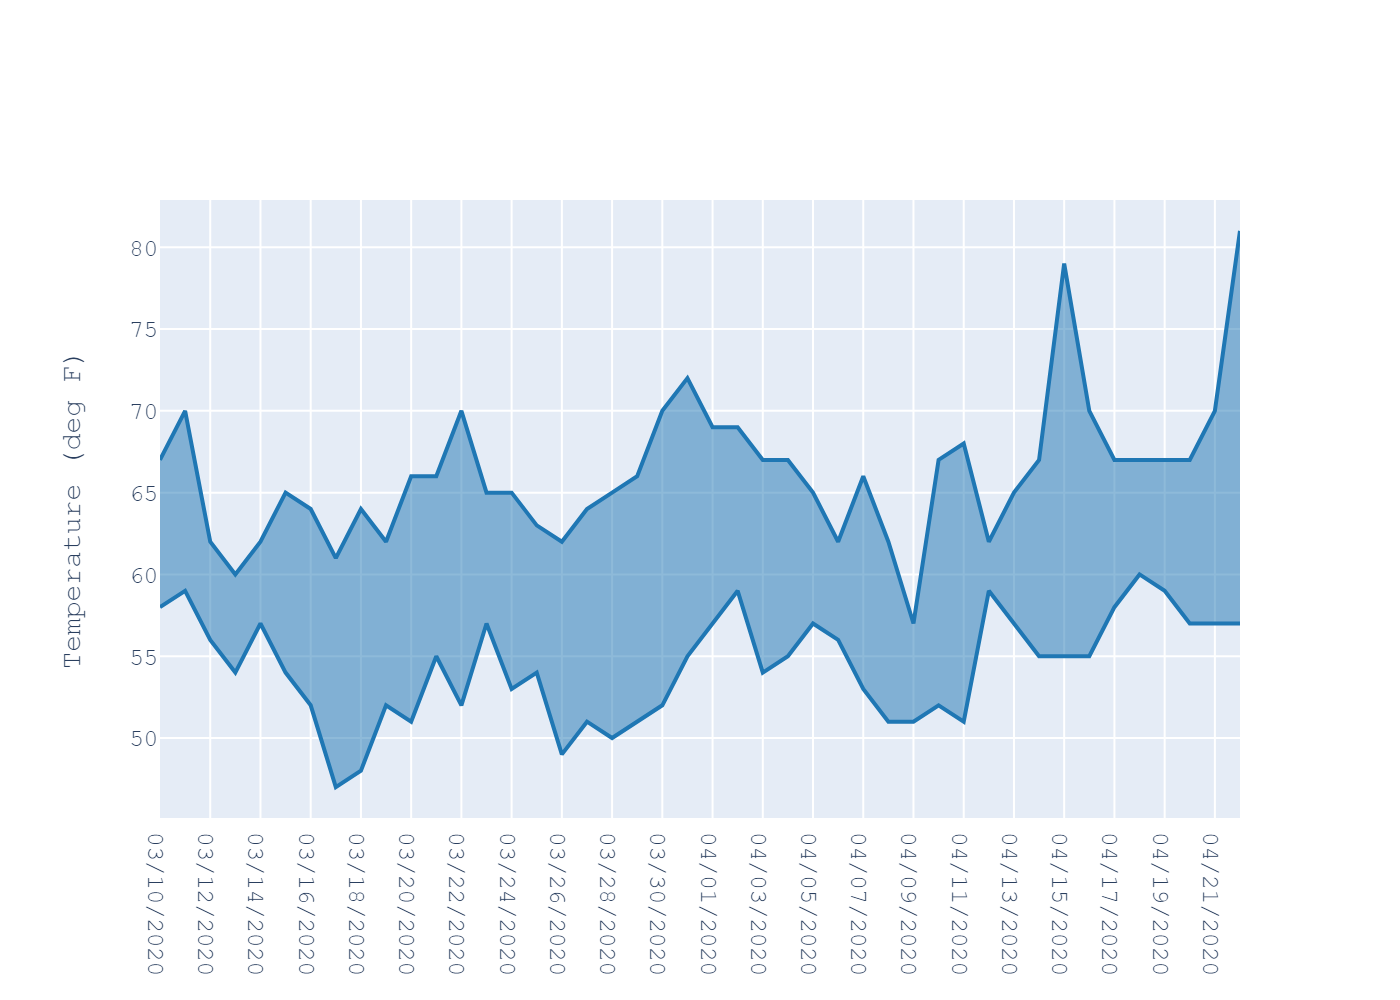
\includegraphics[width=\linewidth]{task4/Louisiana_temp.png}
    \caption{New Orleans Temperature}
  \end{subfigure}

  \begin{subfigure}{0.45\linewidth}
    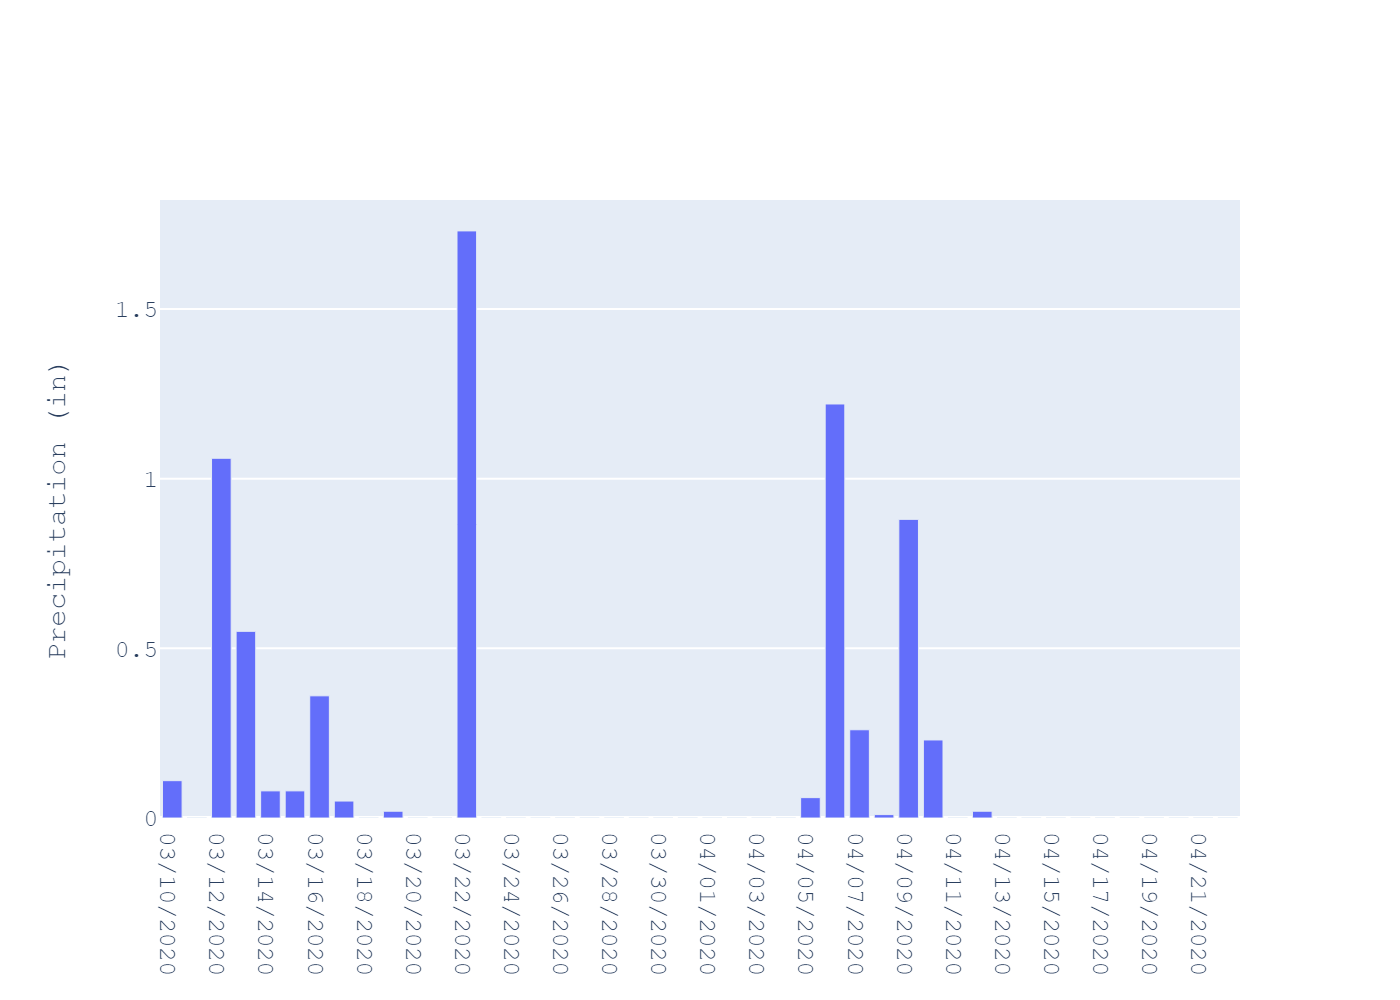
\includegraphics[width=\linewidth]{task4/Louisiana_rain.png}
    \caption{New Orleans Percipitation}
  \end{subfigure}
  \hfil
  \begin{subfigure}{0.45\linewidth}
    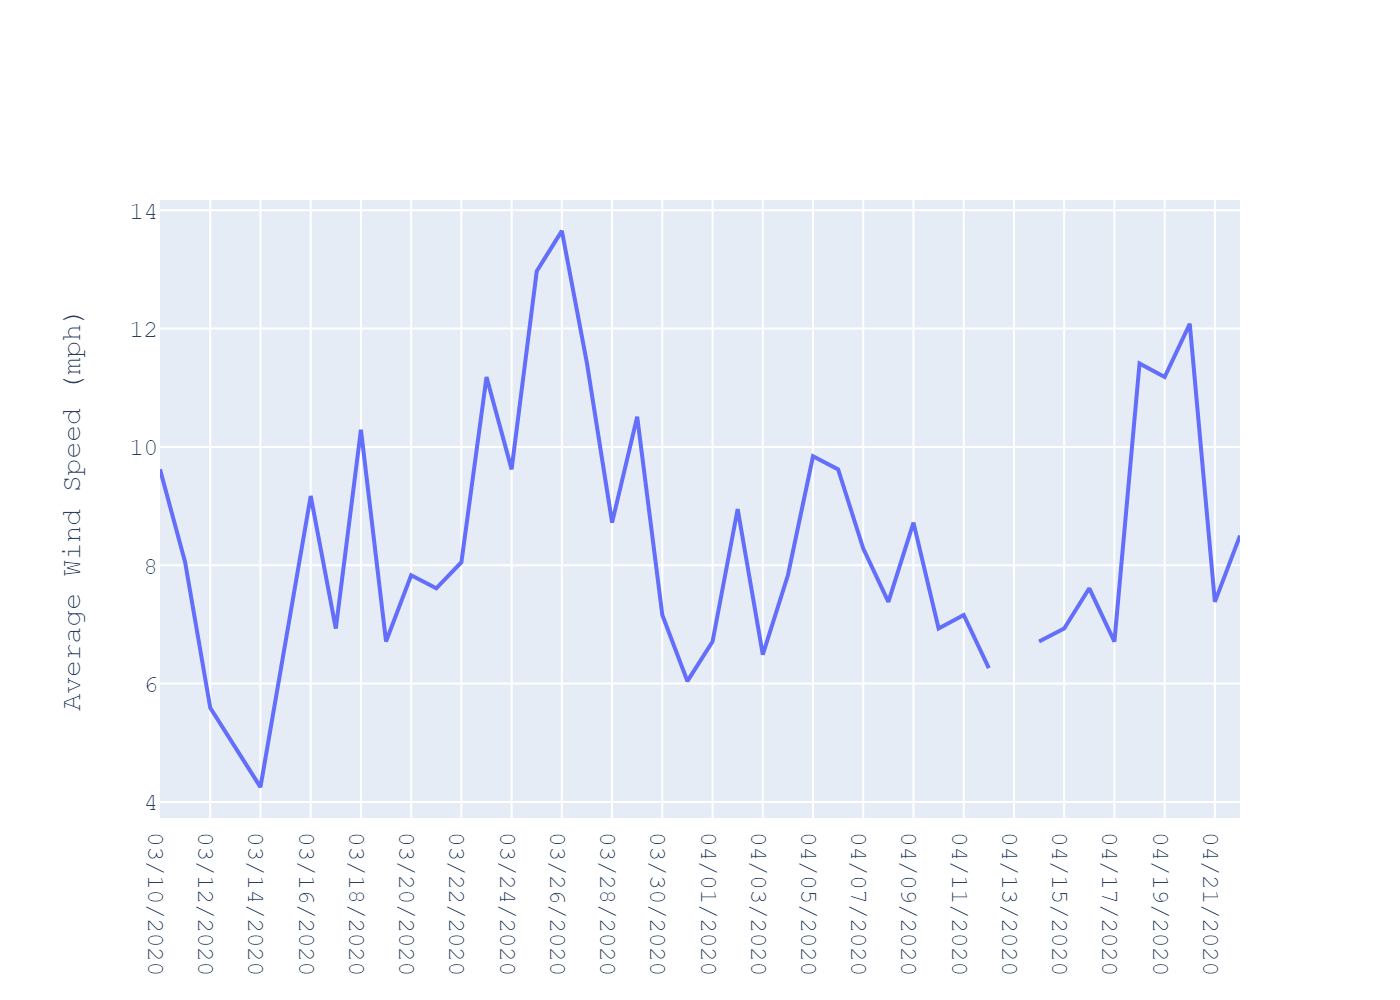
\includegraphics[width=\linewidth]{task4/Louisiana_wnd.png}
    \caption{New Orleans Wind Speed}
  \end{subfigure}

  \caption{Louisiana COVID-19 spread and weather conditions}
  \label{fig:task4CA}
\end{figure}

\begin{table}[H]
  \caption{Correlation between COVID-19 spread and weather conditions in Louisiana}
  \label{Task 4 Louisiana}
  \centering
  \begin{tabular}{lrrrrrr}
\toprule
{} &  Confirmed &    Deaths &      AWND &      PRCP &      TMAX &      TMIN \\
\midrule
Confirmed &   1.000000 &  0.976245 &  0.012217 & -0.137567 &  0.349143 &  0.391529 \\
Deaths    &   0.976245 &  1.000000 &  0.041743 & -0.178289 &  0.430731 &  0.427688 \\
AWND      &   0.012217 &  0.041743 &  1.000000 & -0.118884 & -0.079533 & -0.055577 \\
PRCP      &  -0.137567 & -0.178289 & -0.118884 &  1.000000 & -0.228251 & -0.094460 \\
TMAX      &   0.349143 &  0.430731 & -0.079533 & -0.228251 &  1.000000 &  0.317699 \\
TMIN      &   0.391529 &  0.427688 & -0.055577 & -0.094460 &  0.317699 &  1.000000 \\
\bottomrule
\end{tabular}

\end{table}

\subsection{Analysis}

Based on the studies of the 4 different states listed above, a correlation between temperature and COVID-19 spread cannot be made. Even though there was an approximate 40\% correlation between temperature and confirmed cases, this can be attributed to the fact to seasonal change into the spring as the virus spread in these areas. This also goes against earlier thoughts that warmer temperatures would curb the virus as in-fact, based on the data, the virus is growing as the temperature is increasing.

\newpage
\section{Case Study on New York City}

One of United States' most populous and high-density cities, New York City, is also the current leader for COVID-19 cases and deaths. New York City has made a plethora of information about COVID-19 and other city-related data available to the public. Using the tools developed in the former sections, an analysis has been performed to study the effects of the virus on New York. 

\subsection{Exploration of Data}

Using available New York City zipcode data, a map was generated visualizing the most affected neighborhoods of New York.

\begin{figure}[H]
  \centering
  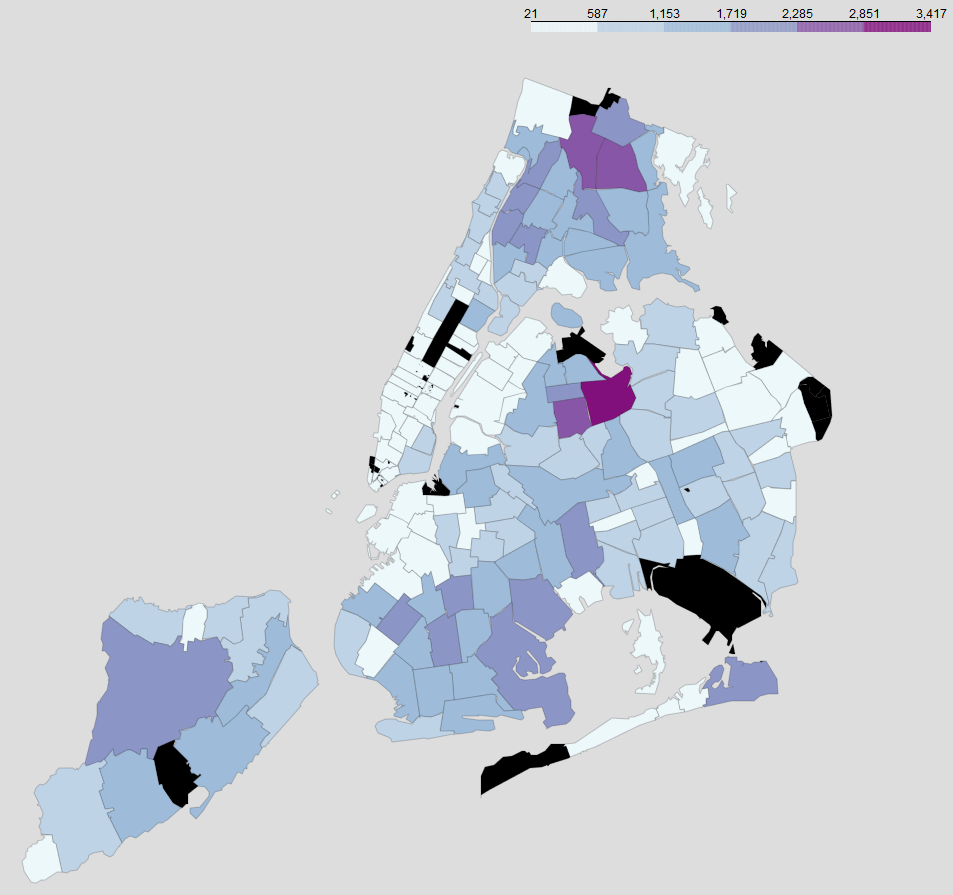
\includegraphics[scale=0.3]{task5/map.PNG}
  \caption{COVID-19 New York City Zipcode Map}
\end{figure}

Analyzing the timeline of confirmed, hospitalized, and death cases in New York City.

\begin{figure}[H]
  \centering
  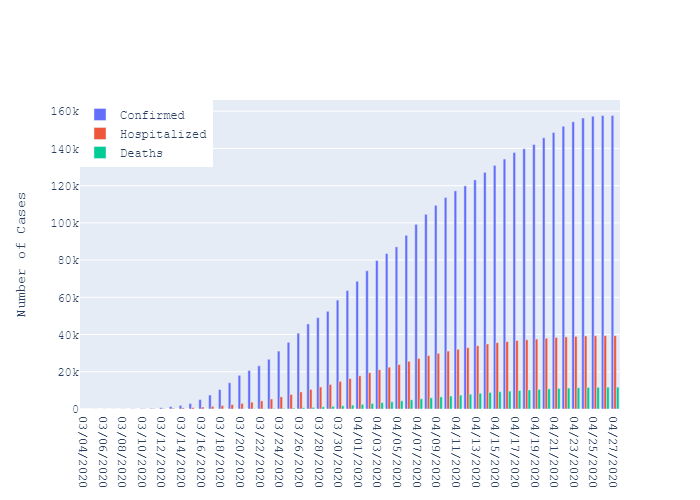
\includegraphics[scale=0.45]{task5/task5_timeline.png}
  \caption{COVID-19 Spread New York City}
\end{figure}

\newpage
\subsection{Correlations for Zipcode Based Data}

Combining datasets on demographic data and train lines based on zipcode with the COVID-19 dataset can provide insight into if any demographic or urban planning attributes correlated with the spread of COVID-19 in that area. 

\begin{table}[H]
  \caption{COVID-19 Correlation in New York City}
  \label{Task 5 Correlation}
  \centering
  \begin{tabular}{lr}
    \toprule
    {Feature}                           & Correlation to Positive Test \\
    \midrule
    % Total Tested                        & 0.975922                     \\
    % Percentage                          & 0.584278                     \\
    % Count Participants                  &  0.399020 \\
    % Count Female                        &  0.362927 \\
    Percent Female                      & 0.381337                     \\
    % Count Male                          &  0.405806 \\
    Percent Male                        & 0.235687                     \\
    % Count Gender Unknown                &       Nan \\
    % Percent Gender Unknown              & Nan                          \\
    % Count Gender Total                  &  0.399020 \\
    % Percent Gender Total                & 0.393472                     \\
    % Count Pacific Islander              &  0.151903 \\
    Percent Pacific Islander            & 0.151903                     \\
    % Count Hispanic Latino               &  0.335900 \\
    Percent Hispanic Latino             & 0.359761                     \\
    % Count American Indian               &  0.252329 \\
    Percent American Indian             & 0.147127                     \\
    % Count Asian Non Hispanic            &  0.031950 \\
    Percent Asian Non Hispanic          & -0.169780                    \\
    % Count White Non Hispanic            &  0.275063 \\
    Percent White Non Hispanic          & 0.310633                     \\
    % Count Black Non Hispanic            &  0.299817 \\
    Percent Black Non Hispanic          & 0.257845                     \\
    % Count Other Ethnicity               &  0.300441 \\
    Percent Other Ethnicity             & 0.113792                     \\
    % Count Ethnicity Unknown             &  0.210921 \\
    Percent Ethnicity Unknown           & 0.057773                     \\
    % Count Ethnicity Total               &  0.399020 \\
    % Percent Ethnicity Total             & 0.393327                     \\
    % Count Permanent Resident Alien      &  0.374101 \\
    Percent Permanent Resident Alien    & 0.112616                     \\
    % Count Us Citizen                    &  0.393106 \\
    Percent US Citizen                  & 0.382285                     \\
    % Count Other Citizen Status          &  0.261078 \\
    Percent Other Citizen Status        & 0.149430                     \\
    % Count Citizen Status Unknown        &       Nan \\
    % Percent Citizen Status Unknown      & Nan                          \\
    % Count Citizen Status Total          &  0.399020 \\
    Percent Citizen Status Total        & 0.393533                     \\
    % Count Receives Public Assistance    &  0.351775 \\
    Percent Receives Public Assistance  & 0.253209                     \\
    % Count Nreceives Public Assistance   &  0.386853 \\
    % Percent Nreceives Public Assistance & 0.350649                     \\
    % Count Public Assistance Unknown     &       Nan \\
    % Percent Public Assistance Unknown   & Nan                          \\
    % Count Public Assistance Total       &  0.399020 \\
    Percent Public Assistance Total     & 0.393472                     \\
    Number of Train Lines               & -0.074779                    \\
    Population                          & 0.821439                     \\
    Population Density                  & 0.017639                     \\
    Housing Units                       & 0.596800                     \\
    Occupied Housing Units              & 0.623721                     \\
    Median Home Value                   & -0.429955                    \\
    Median Household Income             & -0.508028                    \\
    \bottomrule
\end{tabular}

\end{table}

Features such as population and amount of occupied housing units make sense for high correlation. It is interesting to note that the number of train lines in a zipcode and the median household income and home value do not show correlation with confirmed positive tests.

\newpage
\subsection{Predicting the End of COVID-19}

The end results for New York City were using the logarithmic model developed to predict the end results of the pandemic for countries of the world in earlier sections. 

\begin{figure}[H]
  \centering
  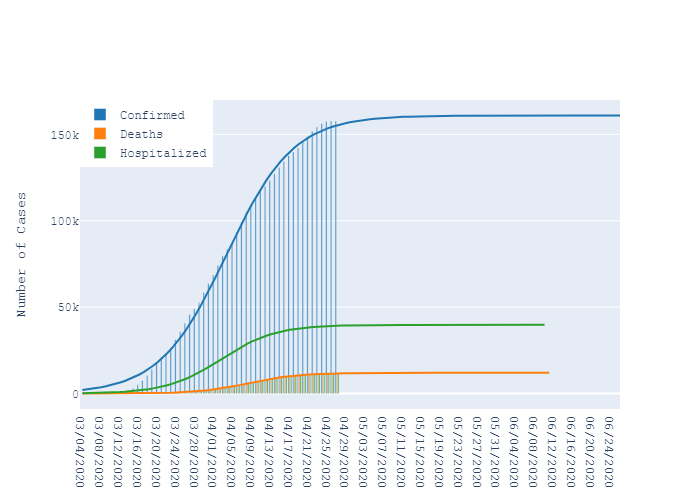
\includegraphics[scale=0.45]{task5/modeling.png}
  \caption{Modeling COVID-19 Spread New York City}
\end{figure}

\begin{table}[H]
  \caption{Results of Modeling New York City}
  \label{Task 5 New York City}
  \centering
  \begin{tabular}{lrrr}
\toprule
   End Date &  Total Confirmed &  Total Hospitalized &  Total Deaths \\
\midrule
 06/26/2020 &           160941 &               39789 &         12005 \\
\bottomrule
\end{tabular}

\end{table}

\newpage
\subsection{Growth Rate Mitigation} 

Calculating and visualizing the growth rate for New York shows that the city managed minimize it to zero. The first case of COVID-19 was confirmed on March 1st. On March 7th, Governor Andrew Cuomo declared a state of emergency and by March 22nd announced a statewide stay in place order after several days of outcries from New York City Mayor Bill de Blasio to do so. Public schools were closed and so were non-essential businesses. Since then, New York City has been challenged with problems of high unemployment, lack of protective equipment and paramedics, testing capabilities, and overcrowding. Even with problems with social distancing for the New York City population, the city managed to lower its growth rate in almost a month. 

\begin{figure}[H]
  \centering
  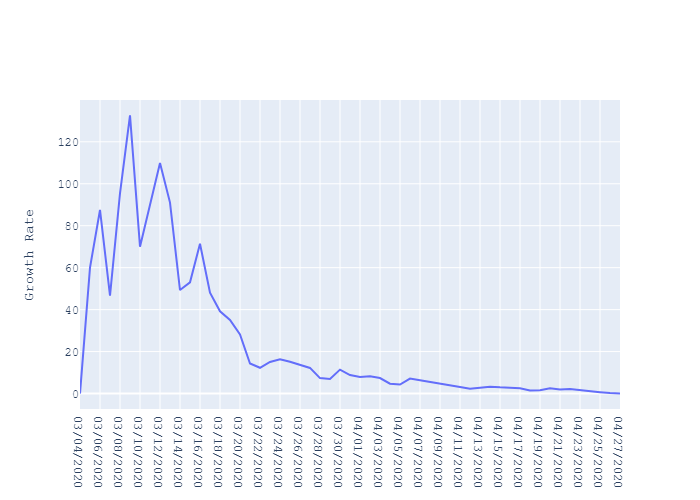
\includegraphics[scale=0.45]{task5/task5_growthrate.png}
  \caption{Modeling COVID-19 Spread New York City}
\end{figure}


\newpage
\section{Conclusion}

The Coronavirus disease 2019 has spread throughout the world quickly, effectively, and metaphorically as it demonstrated the connectivity and interdependence of all countries. The spread of COVID-19 was estimated using different regression models. While a logistic function proved to be the better, but optimistic, predictive model, some countries faced infection amounts closer to the worse-case exponential function. Using the logistic model, the end dates and cases could be predicted. Comparing different mitigation methods between countries showed that governments that were able to control the population early on were able to lower the growth rate quickly. Analyzing New York showed that demographic information could not provide deep insight into the growth of COVID-19 in affected zipcodes but that even in a densely populated city, strong government control could mitigate and lower the virus cases. \\

\newpage
\printbibliography[heading=bibintoc,title={References}]

\end{document}